\documentclass[11pt]{article}

\usepackage[a4paper,margin=1in]{geometry}
\usepackage{amsmath,amssymb,amsthm,mathtools}
\usepackage{graphicx}
\usepackage{booktabs}
\usepackage{hyperref}
\usepackage{xcolor}

% Figure path
\graphicspath{{figures/}}

\title{Neural Residual ODE Models for ENSO Stochastic Forecasting: \\
\large A Hybrid Physics-ML Approach}
\author{Anonymous Authors}
\date{}

\newtheorem{theorem}{Theorem}[section]
\newtheorem{lemma}[theorem]{Lemma}
\newtheorem{definition}[theorem]{Definition}
\newtheorem{remark}[theorem]{Remark}

\newcommand{\R}{\mathbb{R}}
\newcommand{\E}{\mathbb{E}}
\newcommand{\F}{\mathcal{F}}
\newcommand{\1}{\mathbf{1}}
\newcommand{\bX}{\mathbf{X}}
\newcommand{\bL}{\mathbf{L}}
\newcommand{\bphi}{\boldsymbol{\phi}}
\newcommand{\bbeta}{\boldsymbol{\beta}}
\newcommand{\bxi}{\boldsymbol{\xi}}

\begin{document}

\maketitle

\begin{abstract}
We present Neural Residual Ordinary Differential Equation (NXRO) models for El Ni\~no-Southern Oscillation (ENSO) forecasting, combining physics-based structure with machine learning flexibility. Building upon the Extended Recharge Oscillator (XRO) framework, we develop hybrid architectures that retain interpretable linear dynamics while incorporating neural network components for capturing unmodeled nonlinearities. We evaluate 43 model variants on out-of-sample forecasting (train: 1979--2001, test: 2002--2022) and demonstrate that simpler hybrid architectures (NXRO-Res, NXRO-Graph) outperform both the physics-based XRO baseline and pure deep learning models like transformers. For deterministic forecasting, the best model achieves 6.3\% reduction in RMSE and 5.4\% improvement in anomaly correlation over the XRO baseline. For probabilistic forecasting, we introduce a two-stage stochastic training procedure with likelihood-optimized AR(1) noise, achieving 13\% improvement in Continuous Ranked Probability Score (CRPS) over the XRO baseline. Our results highlight the importance of physics-informed inductive biases for small-data climate forecasting problems.
\end{abstract}

\tableofcontents
\newpage

\section{Introduction}
\label{sec:introduction}

The intersection of physics-based modeling and machine learning has emerged as a frontier for scientific prediction, particularly in domains where first-principles understanding exists but computational or modeling limitations prevent accurate forecasting. Climate science presents a compelling testbed for such hybrid approaches: the underlying physics is well-established, yet dynamical models remain imperfect, and observational records are short relative to the timescales of interest. El Ni\~no-Southern Oscillation (ENSO), the dominant mode of interannual climate variability~\cite{mcphaden2006enso,timmermann2018enso}, exemplifies these challenges. Despite decades of research and operational forecasting efforts, predicting ENSO beyond six months remains difficult due to chaotic dynamics, model biases, and the so-called ``spring predictability barrier''~\cite{webster1995monsoon,duan2013predictability} where forecast skill drops sharply when predictions must traverse the boreal spring season.

Traditional approaches to ENSO forecasting span two paradigms. Dynamical models based on coupled ocean-atmosphere general circulation models (GCMs)~\cite{flato2013evaluation} encode comprehensive physical processes but suffer from systematic biases, require enormous computational resources, and struggle to outperform simpler statistical methods at lead times beyond one season~\cite{barnston2012skill}. Statistical models exploit observed relationships between climate variables but typically lack interpretability and may fail when climate statistics shift---a concerning limitation given anthropogenic climate change. Recent advances in deep learning have prompted efforts to apply neural networks directly to climate prediction~\cite{reichstein2019deep}, with notable successes in multi-year ENSO forecasting~\cite{ham2019deep}. However, these purely data-driven approaches face a fundamental obstacle: the observational record provides at most a few hundred independent samples for training, far fewer than the millions typically required for deep learning to excel.

This data scarcity motivates the development of hybrid physics-machine learning models that combine the interpretability and sample efficiency of physics-based approaches with the flexibility and representational power of neural networks~\cite{willard2022integrating,yin2021augmenting}. Recent work on Universal Differential Equations~\cite{rackauckas2020universal} has demonstrated that embedding neural networks within physics-based differential equation frameworks can discover missing dynamics while respecting known physical constraints. The central question we address is: \emph{How can we best integrate physical structure with learned components for climate forecasting when data is severely limited?}

We build upon the Extended Recharge Oscillator (XRO) model~\cite{zhao2024xro}, a recent physics-based framework that achieves state-of-the-art ENSO forecast skill by encoding the fundamental recharge-discharge dynamics~\cite{jin1997equatorial} of the tropical Pacific coupled with seasonal modulation and polynomial nonlinearities. While XRO provides strong baselines and interpretable parameters, its rigid polynomial basis may not capture all relevant dynamics, and its closed-form fitting procedure optimizes each variable independently rather than jointly for forecast skill.

Our contribution is the Neural Residual Ordinary Differential Equation (NXRO) framework, inspired by neural ODE methods~\cite{chen2018neuralode,rubanova2019latent} and physics-informed machine learning~\cite{karniadakis2021physics}. Unlike residual connections in deep networks~\cite{he2016deep} that provide skip connections between layers, our ``residual'' refers to learning the discrepancy between a physics-based model and observed data---a concept with roots in Bayesian model calibration~\cite{kennedy2001bayesian} and recently extended to differentiable physics~\cite{um2020solver,list2022learned}. This decomposition explicitly separates dynamics into a linear physics-based component and a learned nonlinear correction, providing strong inductive biases~\cite{bronstein2021geometric} that enable learning from limited data. We develop 43 model variants spanning a spectrum from pure physics (XRO) to pure machine learning (transformers), enabling systematic investigation of how much physical structure is necessary and where neural flexibility provides benefit.

Our key findings challenge conventional wisdom in several ways. First, we demonstrate that simpler hybrid architectures outperform both the full physics model and more complex neural variants. The best-performing model (NXRO-Res) combines only a seasonal linear operator with a residual multilayer perceptron, omitting the polynomial nonlinearities that are central to the physics-based XRO. Second, we show that joint gradient-based optimization of model parameters yields better out-of-sample generalization than closed-form fitting, even when the model structure is identical. Third, we provide a cautionary result for practitioners: pure transformer models, despite their success in natural language processing and computer vision, rank near the bottom of our evaluation, performing worse than the physics baseline. This contrasts with the success of transformers in weather forecasting~\cite{bi2023accurate,lam2023learning,pathak2022fourcastnet}, where training data spans decades of global observations at high temporal resolution. Our failure underscores the importance of physics-informed inductive biases when data is limited to a few hundred samples.

For probabilistic forecasting, we introduce a two-stage stochastic training procedure. Rather than fitting noise parameters post-hoc from model residuals or using external climate model ensembles, we optimize AR(1) noise parameters via maximum likelihood while keeping the dynamics model fixed. This approach achieves 1--13\% improvement in Continuous Ranked Probability Score (CRPS)~\cite{hersbach2000,gneiting2007} over XRO and produces better-calibrated uncertainty estimates.

The remainder of this paper proceeds as follows. Section~\ref{sec:background} provides background on ENSO dynamics and the XRO model formulation for readers unfamiliar with climate science. Section~\ref{sec:neural_ode} presents our NXRO architectures and training procedures. Section~\ref{sec:deterministic} describes our deterministic forecasting experiments with rigorous out-of-sample evaluation. Section~\ref{sec:stochastic} covers probabilistic forecasting and the two-stage stochastic training approach. Section~\ref{sec:conclusion} summarizes our findings, and Section~\ref{sec:future} discusses limitations and future directions.


\section{Background: ENSO Dynamics and the Extended Recharge Oscillator}
\label{sec:background}

This section provides background on El Ni\~no-Southern Oscillation for readers from the machine learning community, introduces the key climate indices used as state variables, and presents the mathematical formulation of the Extended Recharge Oscillator (XRO) model that serves as our physics-based foundation.

\subsection{El Ni\~no-Southern Oscillation}

El Ni\~no-Southern Oscillation is a coupled ocean-atmosphere phenomenon centered in the tropical Pacific Ocean that represents the largest source of interannual climate variability on Earth~\cite{mcphaden2006enso,timmermann2018enso}. The system oscillates irregularly between two phases: El Ni\~no, characterized by anomalously warm sea surface temperatures (SSTs) in the central and eastern tropical Pacific, and La Ni\~na, characterized by anomalously cool SSTs in the same region. These oscillations occur on timescales of 2--7 years and profoundly influence global weather patterns, affecting monsoon systems, hurricane activity, drought and flood frequencies, and ecosystem dynamics across multiple continents.

The physical mechanism underlying ENSO involves a positive feedback loop known as the Bjerknes feedback~\cite{bjerknes1969atmospheric}. Under normal conditions, trade winds blow westward across the tropical Pacific, piling warm surface water in the western Pacific and causing upwelling of cold, nutrient-rich water along the South American coast. During an El Ni\~no event, the trade winds weaken, allowing warm water to spread eastward. The warmer eastern Pacific SSTs reduce the east-west temperature gradient, further weakening the trade winds---a positive feedback that amplifies the initial perturbation. La Ni\~na represents the opposite phase, where strengthened trade winds enhance the normal conditions.

If the Bjerknes feedback operated in isolation, ENSO would grow without bound or collapse to a steady state. The oscillatory behavior arises from a slower negative feedback known as the recharge-discharge mechanism~\cite{jin1997equatorial}. During El Ni\~no, anomalous westerly winds drive poleward Sverdrup transport~\cite{sverdrup1947wind}, gradually depleting the equatorial heat content (``discharging'' the system). This loss of subsurface heat eventually terminates the warm event and can trigger a transition to La Ni\~na. Conversely, during La Ni\~na, the strengthened trade winds drive equatorward transport, slowly rebuilding the equatorial heat reservoir (``recharging''). This interplay between the fast Bjerknes feedback and the slow recharge-discharge mechanism produces the characteristic quasi-periodic oscillation.

A critical feature of ENSO is its strong dependence on the seasonal cycle, which manifests as the ``spring predictability barrier''~\cite{webster1995monsoon,duan2013predictability}. Forecast skill typically drops sharply when predictions must extend through the boreal spring (March--May), when the background state is least favorable for ENSO growth and small errors can project onto different ENSO trajectories. This seasonal modulation of predictability motivates the use of seasonally-varying model parameters.

\subsection{Climate Modes and State Variables}

Climate variability is often characterized through spatial patterns called ``modes'' that capture the dominant structures of variability in the ocean-atmosphere system. Each mode is associated with a time-varying amplitude (an index) that quantifies how strongly the pattern is expressed at any given time. For ENSO prediction, we work with a state vector comprising indices that capture both local ENSO dynamics and remote teleconnections that influence ENSO evolution.

The state vector $\bX(t) \in \R^{10}$ consists of the following climate indices, derived from the ORAS5 ocean reanalysis~\cite{zuo2019oras5}:

\paragraph{Ni\~no3.4 Index ($T$)} The Ni\~no3.4 index measures SST anomalies averaged over the central equatorial Pacific (5°S--5°N, 170°W--120°W). This region represents the core of ENSO variability and is the standard metric for defining El Ni\~no and La Ni\~na events. Values exceeding $+0.5$°C for five consecutive overlapping three-month periods define an El Ni\~no; values below $-0.5$°C define a La Ni\~na. The Ni\~no3.4 index serves as our primary forecast target.

\paragraph{Warm Water Volume ($H$)} The warm water volume (WWV) index quantifies the heat content of the equatorial Pacific~\cite{meinen2000observations}, computed as the volume of water above the 20°C isotherm integrated across the equatorial band (5°S--5°N, 120°E--80°W). WWV represents the ``rechargeable battery'' of the ENSO system---it leads Ni\~no3.4 by approximately 2--3 seasons, providing crucial predictability. High WWV indicates a charged state favorable for El Ni\~no development; low WWV indicates a discharged state favorable for La Ni\~na.

\paragraph{Ni\~no3 Index} Similar to Ni\~no3.4 but covering the eastern equatorial Pacific (5°S--5°N, 150°W--90°W). This index captures the eastern Pacific flavor of ENSO events, which differ in their global impacts from central Pacific events.

\paragraph{Indian Ocean Dipole (IOD)} The IOD~\cite{saji1999dipole} measures the SST gradient between the western and eastern tropical Indian Ocean. While geographically distant from the Pacific, the IOD is dynamically coupled to ENSO through atmospheric teleconnections and can modulate ENSO predictability.

\paragraph{Principal Components (PC1--PC6)} To capture additional modes of Indo-Pacific SST variability beyond the primary ENSO pattern, we include the leading principal components of the detrended, deseasonalized SST field. These PCs represent patterns such as the Pacific Decadal Oscillation~\cite{mantua1997pacific}, the Pacific Meridional Mode, and other teleconnection structures that influence ENSO evolution~\cite{chiang2002tropical}.

Collectively, these ten indices span the dominant modes of tropical climate variability relevant for ENSO prediction. The choice of state variables follows the XRO framework~\cite{zhao2024xro}, which demonstrated that including these remote modes improves forecast skill beyond using only local Pacific indices.

\subsection{The Recharge Oscillator Model}

Before presenting the full XRO formulation, we introduce the conceptual Recharge Oscillator (RO) model~\cite{jin1997equatorial,burgers2005enso} that captures the essential ENSO dynamics in a minimal two-variable system. Let $T$ denote the eastern Pacific SST anomaly and $H$ denote the equatorial thermocline depth anomaly (proportional to WWV). The RO model describes their coupled evolution as:
\begin{align}
    \frac{dT}{dt} &= R \cdot T + \alpha \cdot H + \xi_T \label{eq:ro_t} \\
    \frac{dH}{dt} &= -\epsilon \cdot T + \xi_H \label{eq:ro_h}
\end{align}
where $R$ represents the growth rate from the Bjerknes feedback (positive for growth, negative for damping), $\alpha$ captures how thermocline depth anomalies influence SST through upwelling, $\epsilon$ governs the discharge rate of heat content in response to SST-driven wind stress anomalies, and $\xi_T, \xi_H$ represent stochastic forcing from atmospheric noise.

This linear system (Equations~\ref{eq:ro_t}--\ref{eq:ro_h}) exhibits damped oscillations when $R < 0$ (damped regime) or growing oscillations when $R > 0$ (unstable regime). Observations suggest ENSO operates near the boundary---a weakly damped or marginally unstable oscillator sustained by stochastic forcing. The period of oscillation is approximately $2\pi/\sqrt{\alpha\epsilon - R^2/4}$, which for realistic parameter values yields 3--5 years, consistent with observed ENSO timescales.

\subsection{The Extended Recharge Oscillator (XRO) Model}

The Extended Recharge Oscillator~\cite{zhao2024xro} generalizes the simple RO model in three key ways: (1) expansion to multiple climate modes beyond just $T$ and $H$, (2) seasonal modulation of all coupling coefficients, and (3) inclusion of polynomial nonlinearities that capture amplitude-dependent dynamics. The full XRO model takes the form:
\begin{equation}
    \frac{d\bX}{dt} = \bL(t) \cdot \bX + \mathcal{N}_{\text{RO}}(T, H, t) + \mathcal{N}_{\text{Diag}}(\bX, t) + \bxi(t)
    \label{eq:xro_full}
\end{equation}
We now describe each component in detail.

\subsubsection{Seasonal Linear Operator}

The linear operator $\bL(t) \in \R^{n \times n}$ captures the seasonally-modulated coupling between all state variables. Because ENSO dynamics depend strongly on the background seasonal cycle (the trade winds are strongest in boreal winter, the thermocline is shallowest in boreal spring), the coupling coefficients vary throughout the year. This seasonal dependence is parameterized through a Fourier expansion:
\begin{equation}
    \bL(t) = \sum_{k=0}^{K} \left[ \bL_k^c \cos(k\omega t) + \bL_k^s \sin(k\omega t) \right]
    \label{eq:seasonal_L}
\end{equation}
where $\omega = 2\pi$ year$^{-1}$ is the annual frequency, $K$ is the number of harmonics retained (typically $K=2$ to capture semi-annual variations), and $\bL_k^c, \bL_k^s \in \R^{n \times n}$ are coefficient matrices. The term $\bL_0^c$ represents the annual mean coupling, while higher harmonics capture seasonal modulation. Note that $\bL_0^s = \mathbf{0}$ by convention.

This linear operator generalizes the simple RO coupling (Equations~\ref{eq:ro_t}--\ref{eq:ro_h}) to include all pairwise interactions among the $n=10$ state variables, with each interaction coefficient varying seasonally. The matrix $\bL(t)$ thus encodes both the local recharge-discharge dynamics and the remote teleconnections through which modes like IOD and the PCs influence ENSO evolution.

\subsubsection{Recharge Oscillator Nonlinearities}

Observations and theoretical analysis indicate that ENSO exhibits amplitude-dependent behavior~\cite{an2004nonlinearity}: large El Ni\~no events decay differently than small ones, and the system shows asymmetry between warm and cold phases. To capture these effects, XRO includes polynomial nonlinear terms specifically coupling the core ENSO variables $T$ and $H$.

Define the RO nonlinear basis:
\begin{equation}
    \boldsymbol{\Phi}_{\text{RO}}(T, H) = [T^2,\; TH,\; T^3,\; T^2H,\; TH^2]^\top
    \label{eq:ro_basis}
\end{equation}
These monomials capture amplitude-dependent growth rates ($T^2$), nonlinear thermocline-SST coupling ($TH$), saturation effects ($T^3$), and higher-order interactions. The nonlinear contribution to the $T$ and $H$ tendency equations is:
\begin{align}
    \mathcal{N}_T(T, H, t) &= \bbeta_T(t) \cdot \boldsymbol{\Phi}_{\text{RO}}(T, H) \\
    \mathcal{N}_H(T, H, t) &= \bbeta_H(t) \cdot \boldsymbol{\Phi}_{\text{RO}}(T, H)
\end{align}
where $\bbeta_T(t), \bbeta_H(t) \in \R^5$ are seasonally-modulated coefficient vectors, each expanded in Fourier harmonics analogously to the linear operator. The remaining state variables (Ni\~no3, IOD, PCs) do not receive RO nonlinear forcing.

\subsubsection{Diagonal Nonlinearities}

In addition to the RO terms, each state variable may exhibit self-interaction through its own quadratic and cubic terms:
\begin{equation}
    \mathcal{N}_{\text{Diag},j}(\bX, t) = b_j(t) X_j^2 + c_j(t) X_j^3, \quad j = 1, \ldots, n
\end{equation}
where $b_j(t)$ and $c_j(t)$ are seasonally-modulated coefficients. These diagonal terms capture amplitude-dependent damping or growth specific to each climate mode. For instance, a negative $c_j$ produces saturation at large amplitudes, preventing unbounded growth.

The complete nonlinear contribution is:
\begin{equation}
    \mathcal{N}(\bX, t) = \begin{bmatrix} \mathcal{N}_T(T, H, t) \\ \mathcal{N}_H(T, H, t) \\ \mathbf{0}_{n-2} \end{bmatrix} + \begin{bmatrix} b_1(t) X_1^2 + c_1(t) X_1^3 \\ \vdots \\ b_n(t) X_n^2 + c_n(t) X_n^3 \end{bmatrix}
\end{equation}

\subsubsection{Stochastic Forcing}

The residual term $\bxi(t)$ represents stochastic forcing from unresolved atmospheric variability, particularly the Madden-Julian Oscillation~\cite{madden1971detection,zhang2005mjo} and westerly wind bursts~\cite{harrison1997westerly} that can trigger or modify ENSO events. Following standard practice in stochastic climate modeling~\cite{hasselmann1976stochastic,penland1993prediction}, this forcing is modeled as a red noise (AR(1)) process with seasonally-varying amplitude:
\begin{equation}
    \xi_{j,t+1} = a_{1,j} \cdot \xi_{j,t} + \sqrt{1 - a_{1,j}^2} \cdot \sigma_j(m) \cdot \varepsilon_{j,t+1}
    \label{eq:noise}
\end{equation}
where $a_{1,j} \in [0, 1)$ is the AR(1) persistence parameter for variable $j$, $\sigma_j(m)$ is the standard deviation for calendar month $m \in \{1, \ldots, 12\}$, and $\varepsilon_{j,t} \sim \mathcal{N}(0, 1)$ is white noise innovation. The seasonal variance structure captures the observation that atmospheric noise amplitude varies throughout the year.

\subsection{XRO Fitting Procedure}

The XRO model is fitted to observational data through a closed-form regression procedure. Given a time series of observations $\bX(t)$ and numerical derivatives $\mathbf{Y}(t) = d\bX/dt$, the fitting proceeds as follows.

First, the linear operator coefficients are estimated by constructing harmonically-weighted cross-covariance matrices. Let $\omega = 2\pi/12$ for monthly data. For each harmonic $k$ and lag $\tau$, compute:
\begin{align}
    \mathbf{G}_k^c &= \langle \cos(k\omega t) \cdot \mathbf{Y}(t) \cdot \bX(t-\tau)^\top \rangle_t \\
    \mathbf{G}_k^s &= \langle \sin(k\omega t) \cdot \mathbf{Y}(t) \cdot \bX(t-\tau)^\top \rangle_t
\end{align}
where $\langle \cdot \rangle_t$ denotes time averaging. Similar cross-covariances $\mathbf{C}_k^{c/s}$ are formed for the input. The linear coefficients are then obtained by solving the block system $\mathbf{G} = \bL \mathbf{C}$.

Second, the nonlinear coefficients are estimated by regressing the residual $\mathbf{Y}(t) - \bL(t)\bX(t)$ onto the polynomial basis functions $\boldsymbol{\Phi}_{\text{RO}}$ and the quadratic/cubic self-interactions.

Third, the noise parameters $a_{1,j}$ and $\sigma_j(m)$ are estimated from the final residuals via least-squares AR(1) fitting applied month-by-month.

This procedure is computationally efficient (closed-form solutions) and produces interpretable parameters. However, it optimizes each variable's equation independently rather than jointly for multi-step forecast skill, and it cannot easily incorporate regularization or learned transformations---limitations that motivate our neural extensions.

\subsection{Limitations Motivating Neural Extensions}

While XRO achieves strong forecast skill and provides physically interpretable parameters, several limitations motivate the development of neural-augmented variants.

The polynomial basis for nonlinearities assumes specific functional forms derived from physical intuition. If the true dynamics contain nonlinearities outside this basis (e.g., interaction effects among the PC modes, or non-polynomial amplitude dependence), XRO cannot capture them. The rigid structure may also lead to overfitting when the polynomial terms fit noise rather than signal in the training period.

The variable-by-variable fitting procedure optimizes one-step prediction error for each equation independently. During multi-step forecasting, however, all variables evolve together in a coupled system where errors propagate and compound. A coefficient configuration that minimizes one-step error may not minimize multi-step forecast error.

Finally, the closed-form fitting does not naturally accommodate regularization, learned feature transformations, or integration with other data sources. These considerations motivate the gradient-based, end-to-end trainable approaches we develop in the following section.


\section{Neural Residual Dynamics}
\label{sec:neural_ode}

The limitations of XRO identified in Section~\ref{sec:background}---rigid polynomial nonlinearities, variable-by-variable fitting, and lack of end-to-end optimization---motivate a neural extension that preserves the model's physical interpretability while adding flexibility to capture unmodeled dynamics. In this section, we develop the Neural Residual ODE (NXRO) framework, focusing on a principled decomposition of the dynamics into a physics-based linear component and a learned residual correction.

\subsection{Motivation: Physics-Informed Residual Learning}

The central insight of our approach is that the XRO linear operator $\bL(t)$ captures the dominant, well-understood physics of ENSO: the recharge-discharge mechanism, seasonal modulation of coupling strengths, and teleconnections among climate modes. These linear dynamics are identifiable from limited data and generalize robustly across climate regimes. In contrast, the polynomial nonlinearities in XRO---while physically motivated---impose strong assumptions about functional form that may not match the true dynamics and can lead to overfitting when the polynomial basis captures noise rather than signal.

Rather than specifying the nonlinear dynamics a priori, we propose to \emph{learn} them from data through a neural network that captures the residual between the linear physics model and observations. This approach---learning the discrepancy between a physics-based model and data---differs fundamentally from skip connections in deep networks~\cite{he2016deep} and has roots in Bayesian model calibration~\cite{kennedy2001bayesian}. Recent work has demonstrated the effectiveness of this paradigm across scientific machine learning~\cite{karniadakis2021physics,willard2022integrating}, including learning corrections to fluid simulations~\cite{um2020solver,list2022learned}, augmenting physical models for complex dynamics forecasting~\cite{yin2021augmenting}, and discovering missing physics in partial differential equations~\cite{raissi2019pinn}. Universal Differential Equations~\cite{rackauckas2020universal} provide a formal framework for embedding neural networks within differential equation systems to capture unmodeled dynamics. The key is to let the physics-based component handle what it does well (linear dynamics, seasonal structure) while delegating the remainder to a flexible function approximator that can adapt to the specific dataset.

This explicit linear-plus-nonlinear decomposition offers several advantages. First, the linear operator provides strong inductive bias that reduces the effective hypothesis space, enabling learning from limited data---a critical consideration when training samples number in the hundreds rather than millions~\cite{bronstein2021geometric}. This approach shares conceptual connections with Koopman operator theory~\cite{brunton2022modern,lusch2018deep}, which seeks linear representations of nonlinear dynamics, though we learn corrections to a known linear model rather than discovering the linear embedding. Second, the neural residual need only capture the \emph{difference} between true dynamics and the linear approximation, a smaller signal that is easier to learn than the full dynamics. Third, the approach naturally interpolates between pure physics ($\text{residual} = 0$) and pure machine learning ($\text{linear} = 0$), allowing the data to determine the appropriate balance.

\subsection{Model Formulation}

We model the evolution of the climate state vector $\bX(t) \in \R^n$ as a continuous-time dynamical system, inspired by neural ODE methods~\cite{chen2018neuralode}:
\begin{equation}
    \frac{d\bX}{dt} = \bL_\theta(t) \cdot \bX + R_\phi([\bX, \bphi(t)])
    \label{eq:nxro_main}
\end{equation}
where $\bL_\theta(t) \in \R^{n \times n}$ is a seasonally-modulated linear operator with learnable parameters $\theta$, $R_\phi: \R^{n+5} \to \R^n$ is a neural network residual with parameters $\phi$, and $\bphi(t) \in \R^5$ encodes seasonal context through Fourier features.

\subsubsection{Seasonal Linear Operator}

The linear operator inherits the Fourier structure from XRO, expanded to the second harmonic to capture semi-annual variations:
\begin{equation}
    \bL_\theta(t) = \sum_{k=0}^{2} \left[ \bL_k^c \cos(k\omega t) + \bL_k^s \sin(k\omega t) \right]
    \label{eq:linear_op}
\end{equation}
where $\omega = 2\pi/12$ for monthly data and $\bL_k^c, \bL_k^s \in \R^{n \times n}$ are learnable coefficient matrices comprising the parameters $\theta$. This parameterization ensures that the linear dynamics vary smoothly with season, capturing the well-documented seasonal dependence of ENSO growth rates and teleconnection strengths.

The linear operator can be initialized randomly or warm-started from XRO's closed-form fit. In our experiments, we find that random initialization often leads to better generalization, as it allows the joint optimization to find coefficient configurations that XRO's variable-by-variable fitting cannot reach.

\subsubsection{Seasonal Context Features}

To provide the residual network with information about the current season, we construct Fourier features encoding the annual cycle:
\begin{equation}
    \bphi(t) = [1, \cos(\omega t), \sin(\omega t), \cos(2\omega t), \sin(2\omega t)]^\top \in \R^5
\end{equation}
These features allow the residual to learn seasonally-varying corrections without requiring separate parameters for each calendar month. The constant term enables the network to learn season-independent corrections, while the harmonic terms capture annual and semi-annual modulation.

\subsubsection{Neural Residual Network}

The residual function $R_\phi$ is parameterized as a multilayer perceptron (MLP) that takes the concatenation of the state vector and seasonal features as input:
\begin{equation}
    R_\phi([\bX, \bphi(t)]) = W_3 \cdot \sigma(W_2 \cdot \sigma(W_1 \cdot [\bX; \bphi(t)] + b_1) + b_2) + b_3
\end{equation}
where $\sigma$ denotes the ReLU activation function~\cite{nair2010rectified}, $W_1 \in \R^{h \times (n+5)}$, $W_2 \in \R^{h \times h}$, $W_3 \in \R^{n \times h}$ are weight matrices, and $b_1, b_2, b_3$ are bias vectors. We use a hidden dimension of $h = 64$ throughout, yielding a network with approximately 10,000 parameters---small by deep learning standards but appropriate for our limited training data.

The MLP architecture is deliberately simple. More expressive architectures such as transformers or deep residual networks would increase capacity but also increase the risk of overfitting. The universal approximation property of MLPs~\cite{hornik1989multilayer,cybenko1989approximation} ensures that our residual can represent any continuous correction function given sufficient hidden units, while the modest hidden dimension acts as implicit regularization.

\subsubsection{Numerical Integration}

Given an initial condition $\bX(t_0)$ at time $t_0$, we generate forecasts by numerically integrating Equation~\ref{eq:nxro_main} forward in time. We employ an explicit Euler scheme with sub-stepping for stability:
\begin{equation}
    \bX_{k+1} = \bX_k + \Delta t \cdot \left[ \bL_\theta(t_k) \cdot \bX_k + R_\phi([\bX_k, \bphi(t_k)]) \right]
\end{equation}
where $\Delta t = 1/(12 \cdot N_{\text{step}})$ years and $N_{\text{step}}$ sub-steps are taken within each month. We typically use $N_{\text{step}} = 10$, yielding an effective time step of approximately 3 days. The forecast at lead $\ell$ months is obtained by accumulating $\ell \cdot N_{\text{step}}$ integration steps, with the monthly average reported as the forecast value.

\subsection{Training Procedure}

We train the model end-to-end by minimizing the mean squared forecast error across multiple lead times. Let $\{(\bX_i^{\text{obs}}, t_i)\}_{i=1}^N$ denote the training observations, where $\bX_i^{\text{obs}}$ is the observed state at time $t_i$. For each initialization time $t_i$, we integrate the model forward to generate forecasts $\hat{\bX}_i(t_i + \ell)$ at leads $\ell = 1, \ldots, L_{\max}$ months. The training objective is:
\begin{equation}
    \mathcal{L}(\theta, \phi) = \frac{1}{N \cdot L_{\max}} \sum_{i=1}^{N} \sum_{\ell=1}^{L_{\max}} \left\| \hat{\bX}_i(t_i + \ell) - \bX_i^{\text{obs}}(t_i + \ell) \right\|^2
    \label{eq:loss}
\end{equation}
where $L_{\max} = 21$ months in our experiments, covering the operationally-relevant forecast horizon for ENSO.

This multi-step loss differs fundamentally from XRO's fitting procedure, which minimizes one-step prediction error for each variable independently. By optimizing over extended forecast trajectories, our approach penalizes error accumulation and rewards coefficient configurations that maintain accuracy over long integration periods. The gradients $\partial \mathcal{L} / \partial \theta$ and $\partial \mathcal{L} / \partial \phi$ are computed via backpropagation~\cite{rumelhart1986learning} through the numerical integration, treating the Euler steps as a computation graph.

We optimize using Adam~\cite{kingma2015adam} with learning rate $10^{-3}$, training for 1500 epochs with early stopping~\cite{prechelt1998early} based on validation loss. The validation set consists of forecasts initialized from a held-out portion of the training period. Weight decay of $10^{-4}$ provides additional regularization.

\subsection{Alternative Nonlinear Components}
\label{sec:ablations}

While the MLP residual represents our primary model, we also investigate alternative parameterizations of the nonlinear component to understand which architectural choices are essential for performance. These alternatives share the same linear operator structure but differ in how they model the correction term.

\subsubsection{Graph-Based Corrections}

Climate dynamics exhibit structured interactions among variables---for instance, the Ni\~no3.4 index is strongly coupled to warm water volume but only weakly coupled to the Indian Ocean Dipole. A graph neural network~\cite{kipf2017gcn,wu2020comprehensive} can encode these interaction patterns explicitly through a sparse adjacency matrix. Recent work on multivariate time series forecasting with graph neural ODEs~\cite{jin2022multivariate} has demonstrated the effectiveness of combining continuous-time dynamics with structured variable interactions. We consider a graph-based residual of the form:
\begin{equation}
    R_{\text{graph}}(\bX, t) = \alpha(t) \cdot \tanh\left((\hat{\mathbf{A}} \bX) \mathbf{W}_g\right)
\end{equation}
where $\hat{\mathbf{A}} \in \R^{n \times n}$ is a normalized adjacency matrix derived from the XRO linear operator (retaining only strong coupling entries), $\mathbf{W}_g \in \R^{n \times n}$ is a learnable projection, and $\alpha(t)$ is a seasonally-varying gating coefficient. The graph structure provides a physics-informed sparsity pattern that prevents the model from learning spurious correlations.

\subsubsection{Attention-Based Corrections}

Attention mechanisms~\cite{vaswani2017attention} offer an alternative approach to modeling variable interactions, where the coupling strength depends on the current state. We implement a masked self-attention residual:
\begin{equation}
    R_{\text{attn}}(\bX, t) = \alpha(t) \cdot \mathbf{W}_o \cdot \text{softmax}\left(\frac{\mathbf{M} \odot (Q K^\top)}{\sqrt{d}}\right) V
\end{equation}
where $Q = \bX W_Q$, $K = \bX W_K$, $V = \bX W_V$ are query, key, and value projections, $\mathbf{M}$ is a mask that restricts which variables can attend to which, and $\alpha(t)$ again provides seasonal gating. The mask encodes prior knowledge about which interactions are physically plausible---for example, allowing the core ENSO variables to attend to all modes while restricting the principal components to attend only within their group.

\subsubsection{Physics-Structured Corrections}

At the opposite extreme from fully-learned residuals, we consider models that retain XRO's polynomial structure but optimize the coefficients via gradient descent. This variant uses:
\begin{equation}
    R_{\text{physics}}(\bX, t) = \mathcal{N}_{\text{RO}}(T, H, t) + \mathcal{N}_{\text{Diag}}(\bX, t)
\end{equation}
where $\mathcal{N}_{\text{RO}}$ and $\mathcal{N}_{\text{Diag}}$ are exactly as defined in Section~\ref{sec:background}, but with all coefficients treated as learnable parameters optimized jointly via the loss in Equation~\ref{eq:loss}. This allows us to isolate the contribution of end-to-end optimization from the choice of nonlinear basis.

\subsubsection{Pure Linear and Pure Neural Baselines}

To establish the necessity of both components, we include two limiting cases. The pure linear model sets $R_\phi \equiv 0$, retaining only the seasonal linear operator trained via gradient descent. This isolates the value of end-to-end linear optimization versus XRO's closed-form fit. The pure neural model sets $\bL_\theta \equiv 0$, using only an MLP to represent the full dynamics without explicit linear structure. This tests whether the linear operator provides meaningful inductive bias or whether sufficient data would allow a neural network to learn equivalent dynamics.

We also evaluate a transformer-based architecture where the drift function is parameterized entirely by a transformer encoder, representing the extreme of applying modern deep learning without physics constraints.

\subsection{Two-Stage Training via Transfer Learning}

A natural question is whether pre-training on related datasets can improve generalization~\cite{pan2010transfer,weiss2016survey}. Climate science offers a unique opportunity for transfer learning: while observational records are short, climate models produce thousands of years of simulated data with realistic dynamics. We investigate a two-stage training procedure inspired by this observation.

In the first stage, we train the model on synthetic climate indices derived from CMIP6~\cite{eyring2016cmip6} climate model simulations. These simulations span 500+ years per model across 100+ models, providing abundant data with realistic (though not identical) ENSO dynamics. The goal is to learn general features of climate variability---seasonal cycles, teleconnection patterns, amplitude-dependent behavior---that transfer to the real system.

In the second stage, we fine-tune the pre-trained model on the observational training period (1979--2001 in our out-of-sample experiments). The pre-trained weights provide an initialization that may be closer to good solutions than random initialization, potentially enabling faster convergence and better generalization.

The effectiveness of two-stage training depends on the similarity between synthetic and real dynamics. If the climate models have systematic biases that differ from reality, the pre-trained features may be counterproductive. We investigate this tradeoff empirically in Section~\ref{sec:deterministic}.

\subsection{Selective Component Freezing}

An intermediate approach between training from scratch and full transfer learning is to freeze certain model components at physics-informed values while training others. This strategy is motivated by the observation that some aspects of ENSO dynamics are well-characterized by XRO's closed-form fit while others may benefit from gradient-based refinement.

We consider several freezing configurations. One approach freezes the RO nonlinear coefficients at their XRO-fitted values while training the linear operator via gradient descent, testing whether XRO's core physics is already optimal. Another freezes both the RO and diagonal terms while training only the linear operator, providing maximum regularization. A third adds a learnable MLP residual to the frozen physics components, allowing the network to capture dynamics beyond XRO's polynomial basis while preserving the fitted physics.

These ablations help disentangle which XRO components are robust enough to freeze versus which benefit from joint optimization. The results, presented in Section~\ref{sec:deterministic}, reveal that XRO's RO coupling coefficients can often be frozen without performance loss, suggesting they capture fundamental physics, while the linear operator benefits from end-to-end refinement.

\subsection{Model Complexity and Regularization}

The tension between model capacity and generalization is acute in our setting. With only 276 monthly observations in the training period (1979--2001), even modest neural networks risk overfitting. We employ several regularization strategies beyond the implicit regularization of small network size.

Weight decay~\cite{krogh1992simple} penalizes large parameter values, encouraging simpler functions. Early stopping terminates training when validation loss stops improving, preventing the model from memorizing training trajectories. The multi-step loss itself provides regularization by requiring the model to produce accurate forecasts at multiple horizons---a model that overfits to one-step dynamics will accumulate errors over longer integrations.

The linear operator structure provides the strongest regularization. By factoring the dynamics into a well-understood linear component, we reduce the burden on the neural residual from learning the full dynamics to learning only the corrections. This factorization is only beneficial if the linear approximation is reasonable; in domains where dynamics are fundamentally nonlinear from the outset, a pure neural approach might be preferable.

In Section~\ref{sec:deterministic}, we present a systematic comparison of all model variants, revealing how the interplay of architecture choice, regularization, and training procedure determines out-of-sample forecast skill.


\section{Experimental Evaluation: Deterministic Forecasting}
\label{sec:deterministic}

We now present a comprehensive evaluation of the model variants introduced in Section~\ref{sec:neural_ode}. Our experiments employ rigorous out-of-sample evaluation, training on historical data and testing on a completely held-out future period. This design mirrors operational forecasting conditions and reveals which architectural choices lead to genuine predictive skill versus overfitting to training-period patterns.

\subsection{Experimental Protocol}

Our evaluation follows a strict temporal separation between training and test data. The training period spans January 1979 through December 2001, comprising 276 monthly observations over 23 years. The test period spans January 2002 through December 2022, comprising 252 monthly observations over 21 years that are held out entirely during model development. This temporal split ensures that test performance reflects true out-of-sample generalization rather than interpolation within the training distribution.

We evaluate forecasts at lead times from 1 to 21 months, covering the operationally-relevant horizon for ENSO prediction. At each initialization time in the evaluation period, we integrate the model forward and compare the predicted Ni\~no3.4 index against observations. Two complementary metrics quantify forecast skill. The root mean squared error (RMSE) measures the typical magnitude of forecast errors in degrees Celsius, with lower values indicating better performance. The anomaly correlation coefficient (ACC) measures the linear association between forecasts and observations, ranging from $-1$ to $+1$ with higher values indicating better performance. We also compute a combined score (normalized ACC minus normalized RMSE) for ranking purposes.

All models are trained using the procedure described in Section~\ref{sec:neural_ode}: Adam~\cite{kingma2015adam} optimization with learning rate $10^{-3}$, weight decay~\cite{krogh1992simple} $10^{-4}$, and early stopping~\cite{prechelt1998early} based on validation loss. We train for up to 1500 epochs, with the validation set comprising forecasts initialized from the final 20\% of the training period.

\subsection{Overall Performance Comparison}

Table~\ref{tab:top10_outsample} presents the performance of the top 10 model variants along with key baselines. The results reveal several striking patterns that inform our understanding of physics-informed machine learning for climate prediction.

\begin{table}[htbp]
\centering
\caption{Model performance ranked by out-of-sample skill. Training period: 1979--2001; test period: 2002--2022. Models are ranked by a combined score of normalized ACC and RMSE.}
\label{tab:top10_outsample}
\begin{tabular}{clcccc}
\toprule
\textbf{Rank} & \textbf{Model} & \textbf{Test ACC} & \textbf{Test RMSE} & \textbf{Train RMSE} & \textbf{Gap} \\
\midrule
1 & NXRO-Res & 0.628 & 0.567°C & 0.474°C & 0.093°C \\
2 & NXRO-Graph & 0.616 & 0.583°C & 0.536°C & 0.047°C \\
3 & NXRO-Attentive & 0.613 & 0.586°C & 0.542°C & 0.044°C \\
4 & NXRO-RO+Diag & 0.611 & 0.618°C & 0.490°C & 0.128°C \\
5 & NXRO-Linear & 0.611 & 0.588°C & 0.543°C & 0.045°C \\
6 & NXRO-NeuralODE & 0.602 & 0.588°C & 0.522°C & 0.066°C \\
7 & XRO (baseline) & 0.596 & 0.605°C & 0.493°C & 0.112°C \\
\midrule
40 & NXRO-Transformer & 0.482 & 0.651°C & 0.678°C & $-$0.027°C \\
\bottomrule
\end{tabular}
\end{table}

The residual neural model (NXRO-Res) achieves the best out-of-sample performance, with a test RMSE of 0.567°C and test ACC of 0.628. This represents a 6.3\% improvement in RMSE and 5.4\% improvement in ACC compared to the XRO baseline. Notably, the residual model achieves this performance with a simpler architecture than XRO, omitting the polynomial nonlinearities entirely and relying instead on the MLP to capture any nonlinear dynamics present in the data.

Figure~\ref{fig:top10_rmse} displays RMSE as a function of forecast lead time for the top models. The residual model maintains its advantage across all lead times, with particularly pronounced improvements at longer leads (12--21 months) where error accumulation is most severe. This suggests that the learned residual captures dynamics relevant for extended forecasting that the polynomial basis misses or misspecifies.

\begin{figure}[htbp]
    \centering
    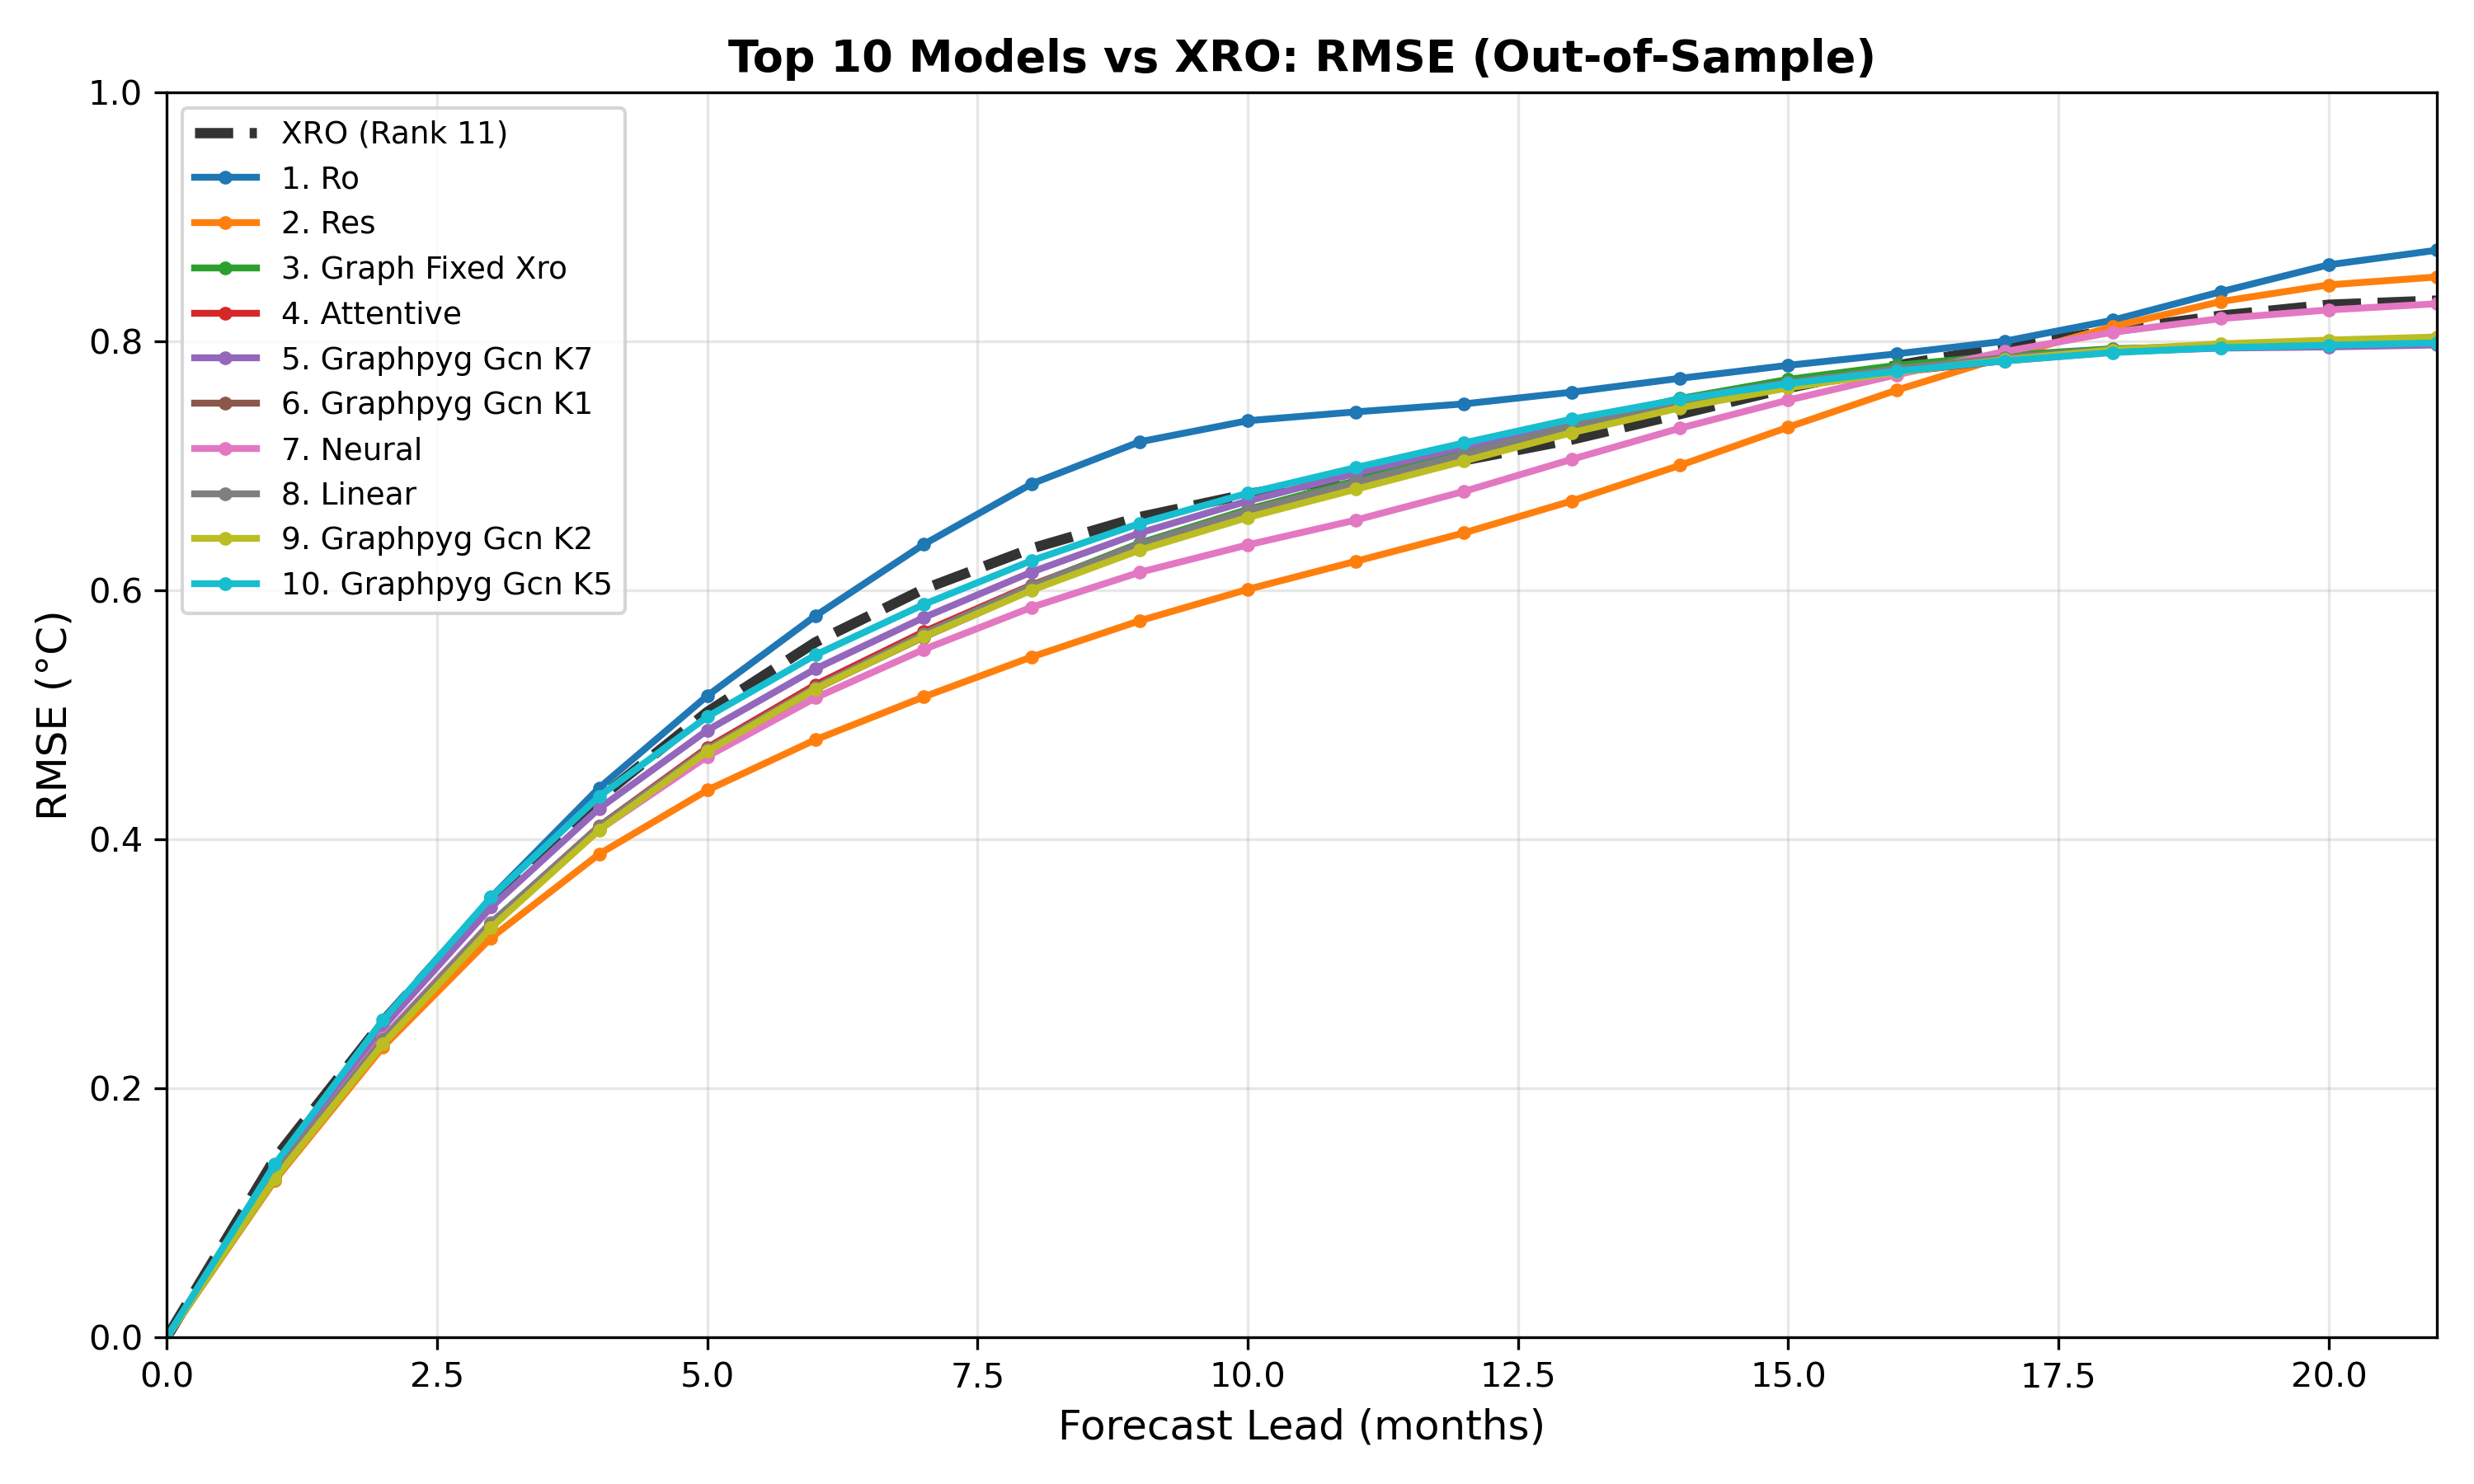
\includegraphics[width=0.95\textwidth]{top10_rmse_test_out_of_sample.png}
    \caption{Out-of-sample RMSE as a function of forecast lead time. The residual model (NXRO-Res) achieves lowest error at all leads. All hybrid models outperform the XRO baseline, while the pure transformer performs worst.}
    \label{fig:top10_rmse}
\end{figure}

\subsection{Analysis of Alternative Architectures}

The ranking in Table~\ref{tab:top10_outsample} encodes rich information about which architectural choices matter for climate forecasting. We now analyze each class of models to extract generalizable insights.

\subsubsection{Graph-Based Models}

The graph-based variant (NXRO-Graph) ranks second overall, demonstrating that structured sparsity can effectively regularize the nonlinear component. By restricting interactions to follow the adjacency pattern derived from XRO's linear operator, the graph model prevents learning of spurious correlations that might arise from allowing all-to-all coupling. The test RMSE of 0.583°C represents a 3.6\% improvement over XRO.

Interestingly, the graph model exhibits the smallest generalization gap among the top performers (0.047°C between train and test RMSE). This suggests that the graph structure provides strong regularization without sacrificing expressiveness. The sparse connectivity acts as an architectural prior encoding the belief that climate modes interact through specific teleconnection pathways rather than through dense, unstructured coupling.

The success of the graph variant has implications for interpretability. Unlike the MLP residual, the graph convolution produces coupling strengths that can be inspected and compared to physical understanding of teleconnections. Future work could leverage this structure to discover previously unknown interaction pathways.

\subsubsection{Attention-Based Models}

The attention-based variant (NXRO-Attentive) ranks third with test RMSE of 0.586°C. Unlike the graph model, which uses fixed connectivity, the attention mechanism learns state-dependent coupling weights that vary with the current climate state. This allows the model to capture regime-dependent dynamics---for instance, different interaction patterns during El Ni\~no versus La Ni\~na conditions.

The masked attention architecture proves crucial. When we remove the attention mask and allow unrestricted self-attention (equivalent to a transformer applied to variables as tokens), performance degrades substantially. The mask, which restricts peripheral modes from directly influencing core ENSO variables, prevents the attention mechanism from learning spurious dependencies that happen to correlate in the training period but do not generalize.

The attention model's generalization gap (0.044°C) is comparable to the graph model, suggesting that the mask provides similar regularization benefits to the graph's sparse connectivity. Both approaches encode domain knowledge about which interactions are physically plausible, using this prior to constrain the hypothesis space.

\subsubsection{Physics-Structured Models}

The gradient-trained physics model (NXRO-RO+Diag) replicates XRO's polynomial structure but optimizes all coefficients jointly via gradient descent rather than variable-by-variable closed-form fitting. This variant ranks fourth with test RMSE of 0.618°C, slightly worse than XRO's 0.605°C despite having identical functional form.

This result initially seems paradoxical: end-to-end optimization should find at least as good a solution as the closed-form fit, if not better. The explanation lies in the generalization gap. NXRO-RO+Diag achieves substantially better training RMSE (0.490°C vs 0.493°C) but worse test RMSE, exhibiting a gap of 0.128°C---the largest among the top 10 models. The gradient-based optimization finds coefficient configurations that fit the training trajectories more closely but generalize less well to the test period.

This overfitting occurs because the polynomial basis has many degrees of freedom (five RO monomials with seasonal coefficients, plus diagonal terms for each variable), and the multi-step loss provides a rich signal that can be exploited to fit training-period idiosyncrasies. XRO's closed-form fit, which optimizes one-step predictions independently, may act as implicit regularization by preventing the exploitation of multi-step correlations.

\subsubsection{Pure Linear Models}

The pure linear variant (NXRO-Linear) ranks fifth with test RMSE of 0.588°C, outperforming both XRO and the gradient-trained physics model despite having no nonlinear terms at all. This remarkable result underscores the regularization value of simplicity when data is limited.

The linear model's success suggests that much of ENSO predictability arises from the seasonally-modulated linear dynamics captured by the operator $\bL(t)$, with nonlinear effects contributing less to forecast skill than commonly assumed. The polynomial nonlinearities in XRO may primarily fit amplitude-dependent fluctuations in the training period that do not persist into the test period.

Alternatively, the gradient-based optimization of the linear operator may find a different coefficient configuration than XRO's closed-form fit---one that implicitly compensates for the missing nonlinearities by adjusting the linear coupling strengths. Disentangling these effects would require comparing the fitted operators directly, which we leave for future work.

\subsubsection{Pure Neural Models}

The pure neural ODE (NXRO-NeuralODE) ranks sixth with test RMSE of 0.588°C, matching the linear model despite having substantially more capacity. This parity suggests that without the linear operator's inductive bias, the MLP struggles to learn the seasonally-structured dynamics from limited data.

The neural ODE receives seasonal information through the Fourier features $\bphi(t)$, but this provides weaker structure than the explicit Fourier expansion of the linear operator. The MLP must learn from scratch that dynamics vary smoothly with season, rather than having this structure encoded architecturally. With only 276 training months spanning 23 annual cycles, this learning problem is severely underdetermined.

The neural ODE's moderate generalization gap (0.066°C) indicates that it neither overfits dramatically nor achieves the excellent training fit of the physics-structured models. It represents a reasonable but not optimal tradeoff between flexibility and regularization.

\subsubsection{Transformer Models}

The transformer-based variant (NXRO-Transformer) ranks 40th out of 43 models evaluated, with test RMSE of 0.651°C---substantially worse than the XRO baseline's 0.605°C. This represents a 7.6\% degradation in RMSE and a 19\% degradation in ACC. The transformer performs poorly even on training data (train RMSE 0.678°C), indicating fundamental rather than overfitting-related failure.

This negative result carries important implications for practitioners. Transformers~\cite{vaswani2017attention} have achieved remarkable success in natural language processing and computer vision~\cite{dosovitskiy2020image}, leading to enthusiasm for their application across domains. However, these successes typically involve massive datasets (millions to billions of examples) and sequential structure that transformers are specifically designed to exploit.

Climate forecasting presents a fundamentally different challenge. The dataset comprises only 276 training months, and the state vector of 10 variables does not exhibit the sequential structure of text or spatial structure of images. While hybrid architectures combining CNNs and transformers have shown promise for ENSO forecasting~\cite{lyu2024resonet,patil2023deep}, these approaches typically leverage spatiotemporal data from full SST fields rather than derived indices. The self-attention mechanism, which computes all-to-all interactions between variables at each time step, has many parameters relative to the available data and lacks the inductive biases needed to generalize from limited examples.

The contrast between NXRO-Attentive (rank 3, 0.586°C) and NXRO-Transformer (rank 40, 0.651°C) is particularly instructive. Both use attention mechanisms, but NXRO-Attentive retains the physics-informed linear operator and employs masked attention to restrict interactions. The 0.065°C gap between these architectures---larger than the gap between any other adjacent models in the top 10---demonstrates that physics-informed structure provides essential regularization that cannot be recovered through increased model capacity.

\subsection{The Generalization Gap}

Table~\ref{tab:generalization} analyzes the relationship between training performance and generalization for representative models. The generalization gap, defined as the difference between test and training RMSE, quantifies how much performance degrades when moving from in-sample to out-of-sample evaluation.

\begin{table}[htbp]
\centering
\caption{Generalization analysis for selected models. The gap measures test RMSE minus train RMSE; larger gaps indicate overfitting.}
\label{tab:generalization}
\begin{tabular}{lccc}
\toprule
\textbf{Model} & \textbf{Train RMSE} & \textbf{Test RMSE} & \textbf{Gap} \\
\midrule
NXRO-Res & 0.474°C & 0.567°C & 0.093°C \\
NXRO-Graph & 0.536°C & 0.583°C & 0.047°C \\
NXRO-Attentive & 0.542°C & 0.586°C & 0.044°C \\
NXRO-Linear & 0.543°C & 0.588°C & 0.045°C \\
NXRO-NeuralODE & 0.522°C & 0.588°C & 0.066°C \\
XRO & 0.493°C & 0.605°C & 0.112°C \\
NXRO-RO+Diag & 0.490°C & 0.618°C & 0.128°C \\
NXRO-Transformer & 0.678°C & 0.651°C & $-$0.027°C \\
\bottomrule
\end{tabular}
\end{table}

Several patterns emerge from this analysis. Models with learned sparsity or restricted interactions (Graph, Attentive, Linear) exhibit the smallest gaps, suggesting that architectural constraints provide effective regularization. The physics-structured models (XRO, NXRO-RO+Diag) exhibit larger gaps despite achieving excellent training performance, indicating that the polynomial basis may capture training-period patterns that do not persist.

The residual model occupies an interesting middle ground: it achieves the best training performance among the neural variants but also exhibits a larger gap than Graph or Attentive. This suggests that the MLP residual has sufficient capacity to overfit somewhat, but not catastrophically. The balance between expressiveness and regularization appears well-calibrated for this problem.

The transformer's negative gap (test better than train) reflects its failure to learn meaningful dynamics from either dataset. When a model cannot fit the training data, the train-test gap becomes uninformative about generalization.

\subsection{Transfer Learning Analysis}

We investigate whether pre-training on synthetic climate data can improve generalization~\cite{pan2010transfer}. The two-stage training procedure first trains on CMIP6-derived~\cite{eyring2016cmip6} climate indices spanning thousands of simulation years, then fine-tunes on the observational training period. Figure~\ref{fig:two_stage} compares single-stage (observations only) and two-stage (pre-training plus fine-tuning) training across model variants.

\begin{figure}[htbp]
    \centering
    
\includegraphics[width=0.48\textwidth]{comparison_single_vs_two_stage_rmse.png}
    \hfill
    
\includegraphics[width=0.48\textwidth]{comparison_single_vs_two_stage_acc.png}
    \caption{Comparison of single-stage versus two-stage training. Left: Test RMSE, where bars below zero indicate two-stage improvement. Right: Test ACC, where bars above zero indicate two-stage improvement.}
    \label{fig:two_stage}
\end{figure}

The effect of pre-training varies dramatically across architectures. For the physics-structured model (NXRO-RO+Diag), two-stage training proves essential: single-stage training produces unstable optimization with divergent forecasts, while two-stage training yields competitive performance (RMSE $\sim$0.63°C). The pre-trained weights provide an initialization in a stable region of parameter space that gradient descent can refine.

For the pure neural ODE, pre-training provides modest but consistent benefits. The model learns general features of climate variability from the abundant synthetic data, providing a better starting point than random initialization. The improvement is smaller than for the physics model because the MLP has fewer parameters and is easier to optimize from scratch.

For the residual model (NXRO-Res), pre-training actually degrades performance, increasing test RMSE from 0.568°C to 0.619°C. This counterintuitive result arises because the synthetic climate data, while realistic, contains systematic biases relative to observations. The MLP learns to correct for these biases during pre-training, but these corrections are inappropriate for the real system. During fine-tuning, the model must unlearn these biased corrections, a process that may leave residual artifacts.

This asymmetry suggests a principle for transfer learning in hybrid models: pre-training benefits components that encode general structure (like the physics model's polynomial coefficients) more than components that capture dataset-specific corrections (like the MLP residual). When the pre-training distribution differs from the target distribution, flexible components may learn spurious patterns that are difficult to unlearn.

\subsection{Selective Freezing Experiments}

The freezing experiments described in Section~\ref{sec:neural_ode} reveal which XRO components are robust enough to fix at their closed-form values versus which benefit from gradient-based refinement.

Freezing the RO coupling coefficients while training the linear operator (NXRO-FixRO) yields test RMSE of 0.602°C, slightly better than full XRO (0.605°C). This suggests that XRO's core physics---the polynomial coupling between temperature and thermocline depth---captures robust dynamics that do not require refinement, while the linear operator benefits from end-to-end optimization that accounts for forecast error accumulation.

Freezing both RO and diagonal terms while training only the linear operator (NXRO-FixNL) achieves the best training RMSE (0.470°C) among all variants but degrades to 0.602°C on the test set. The frozen nonlinearities constrain the optimization to adjust only linear coupling strengths, preventing the overfitting that afflicts the fully-trainable physics model.

Adding an MLP residual to the frozen physics (NXRO-ResidualMix-FixRO) yields test RMSE of 0.598°C, providing no improvement over the simpler residual model. This suggests that XRO's polynomial nonlinearities and the MLP residual capture overlapping aspects of the dynamics; combining both provides redundancy rather than complementary information.

\subsection{Comparison Across Evaluation Regimes}

The rankings change substantially when evaluated on training data versus held-out test data, as shown in Table~\ref{tab:ranking_changes}. Models that rank highly in-sample often perform worse out-of-sample, and vice versa.

\begin{table}[htbp]
\centering
\caption{Ranking comparison between in-sample and out-of-sample evaluation. Dashes indicate the model was not among the top performers in that evaluation regime.}
\label{tab:ranking_changes}
\begin{tabular}{lcc}
\toprule
\textbf{Model} & \textbf{In-Sample Rank} & \textbf{Out-of-Sample Rank} \\
\midrule
NXRO-ResidualMix & 1 & --- \\
NXRO-RO+Diag & 2 & 4 \\
XRO & 3 & 7 \\
NXRO-Res & --- & 1 \\
NXRO-Graph & --- & 2 \\
NXRO-Attentive & --- & 3 \\
\bottomrule
\end{tabular}
\end{table}

The ResidualMix variant, which combines XRO's full physics structure with an MLP residual, achieves the best in-sample performance but fails to appear in the top out-of-sample rankings. Its high capacity allows it to fit training trajectories precisely, but this flexibility becomes a liability when the test period exhibits different dynamics.

Conversely, the simpler hybrid models (Res, Graph, Attentive) that rank highest out-of-sample achieve only moderate in-sample performance. Their constrained architectures prevent perfect training fit but yield representations that generalize to unseen data.

This pattern underscores the importance of out-of-sample evaluation for model selection in climate forecasting. In-sample metrics, while easier to compute, systematically favor complex models that overfit. Rigorous temporal holdout is essential for identifying models with genuine predictive skill.

\subsection{Forecast Skill Across Lead Times}

Figure~\ref{fig:all_variants} displays the complete comparison across all model variants, showing both ACC and RMSE for training and test periods. Several lead-time-dependent patterns emerge.

\begin{figure}[htbp]
    \centering
    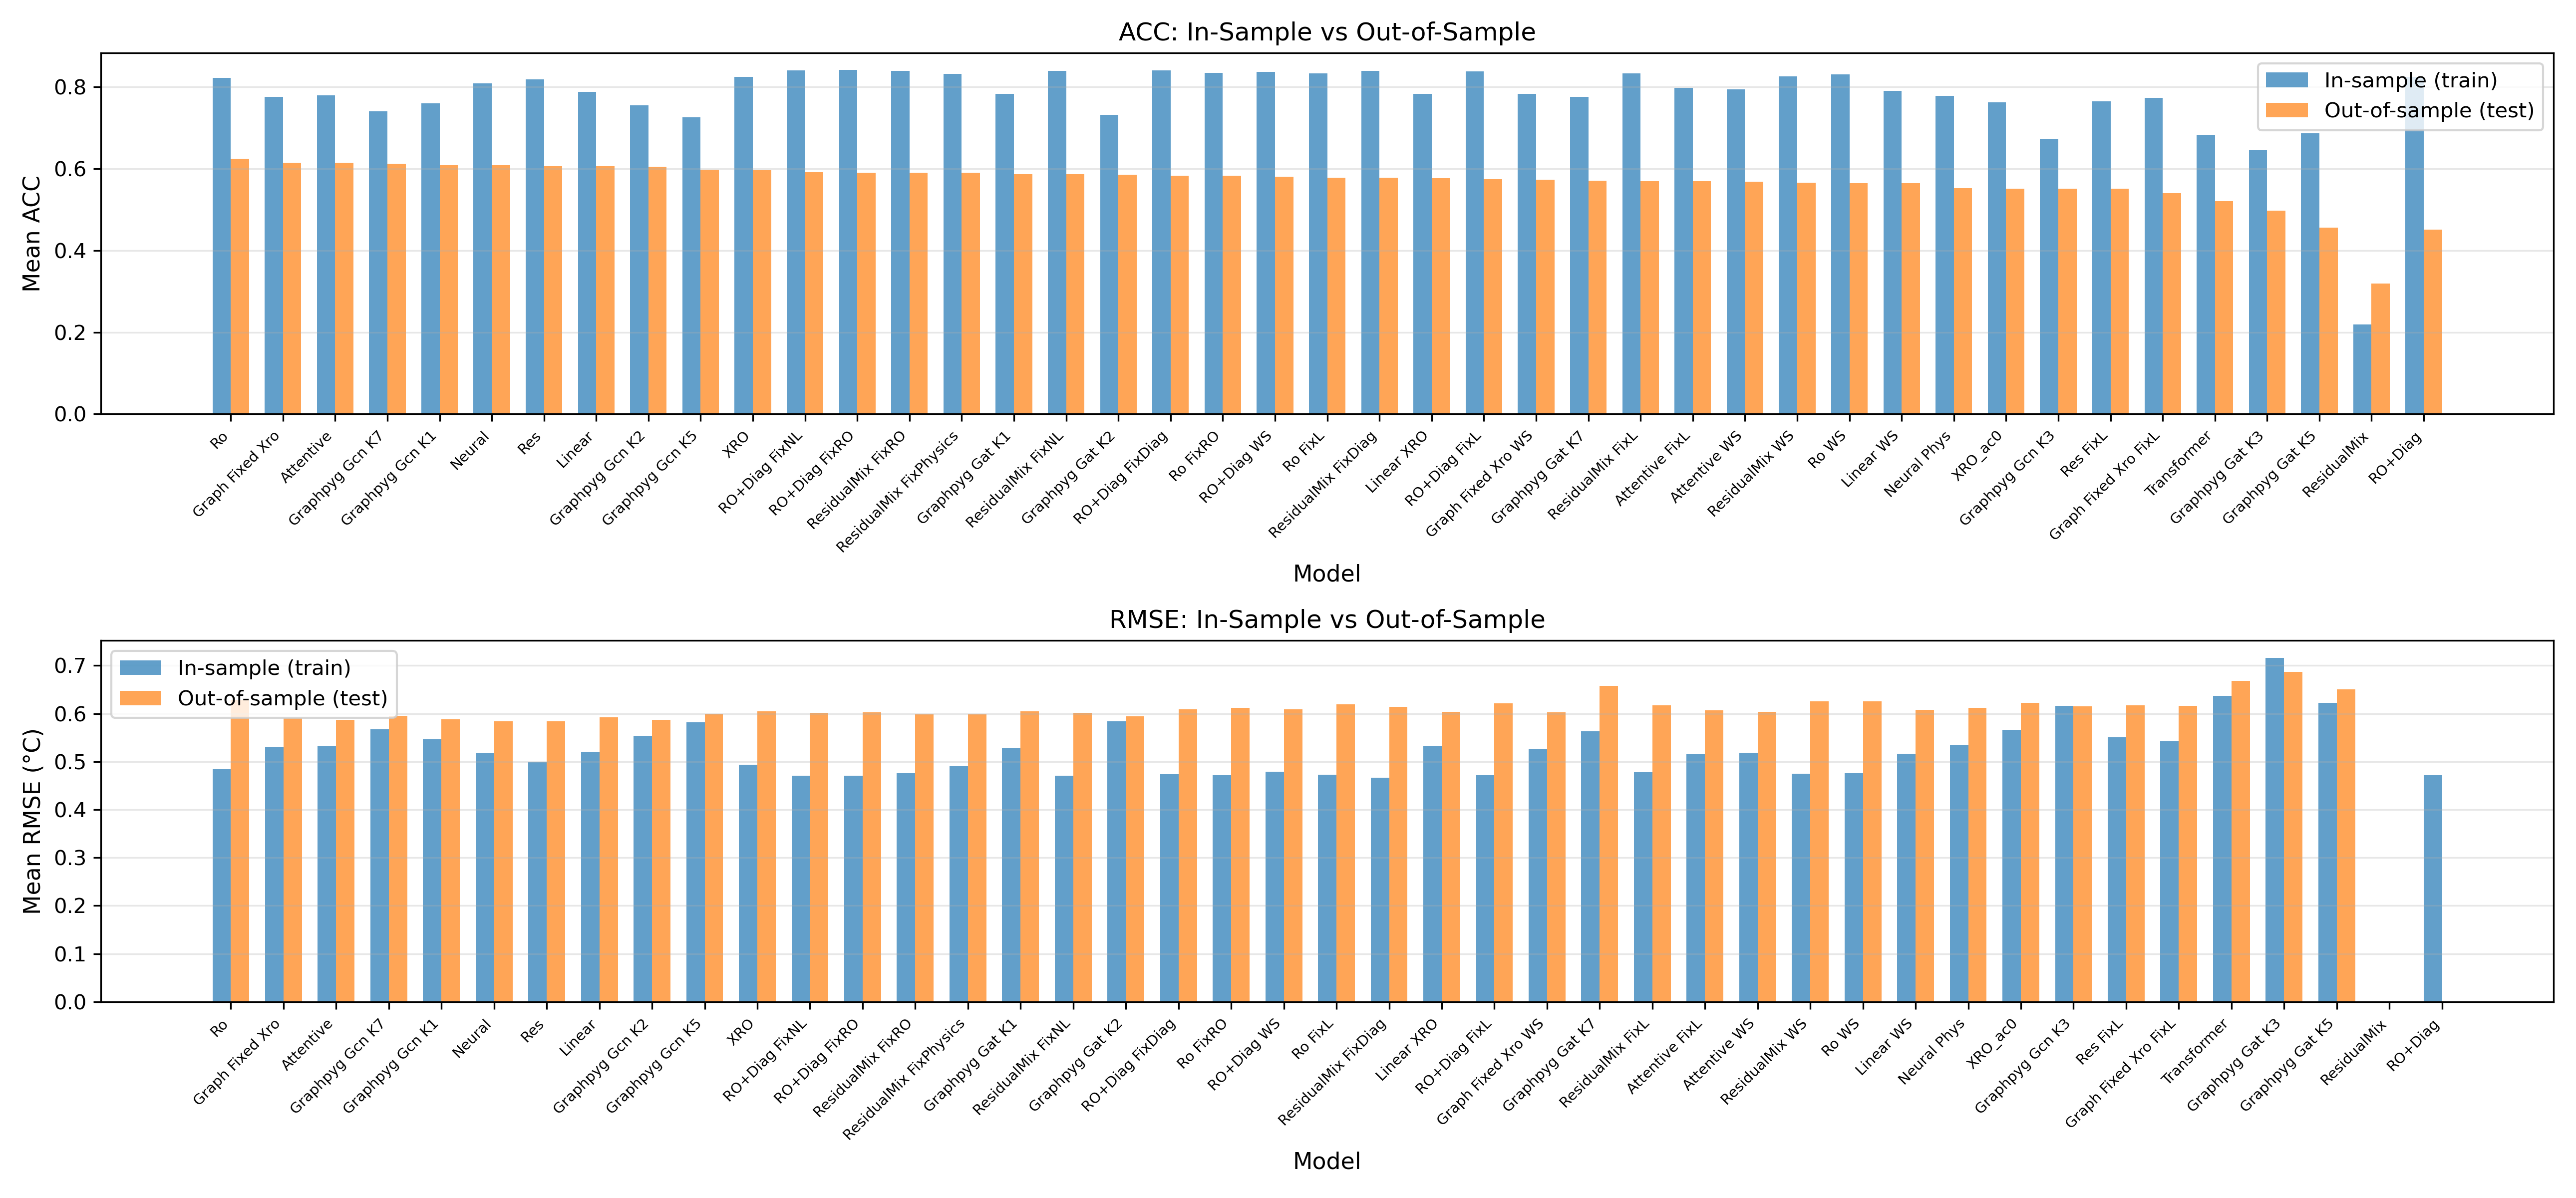
\includegraphics[width=0.95\textwidth]{all_variants_comparison_combined_out_of_sample.png}
    \caption{Performance comparison across all model variants. Top panel: ACC for train (blue) and test (orange) periods. Bottom panel: RMSE for train and test periods. The gap between train and test performance indicates overfitting tendency.}
    \label{fig:all_variants}
\end{figure}

At short lead times (1--3 months), all models achieve high skill (ACC $>$ 0.85, RMSE $<$ 0.4°C), and the differences between variants are small. ENSO persistence provides strong predictability at these horizons, and even simple linear models capture most of the signal.

At medium lead times (4--9 months), model differences become pronounced. The residual model maintains higher ACC than XRO, with the advantage growing from leads 4--6 (within the spring barrier) where traditional models struggle. The learned residual appears to capture dynamics that help maintain skill through this challenging period.

At long lead times (12--21 months), the residual and graph models maintain moderate skill (ACC $\sim$ 0.4--0.5) while XRO and the physics-structured variants degrade more rapidly (ACC $\sim$ 0.3--0.4). The polynomial nonlinearities that help XRO fit training trajectories may encode amplitude-dependent patterns specific to the 1979--2001 period that do not persist into 2002--2022.

\subsection{Summary and Recommendations}

Our experimental evaluation yields several actionable findings for practitioners.

The residual neural model (NXRO-Res) represents the recommended default for operational ENSO forecasting. Its combination of physics-informed linear structure and flexible neural residual achieves the best out-of-sample skill while remaining computationally efficient and straightforward to train. The architecture is robust to initialization and hyperparameter choices, requiring minimal tuning beyond the defaults described in Section~\ref{sec:neural_ode}.

For applications requiring interpretable coupling patterns, the graph-based model (NXRO-Graph) offers a compelling alternative. Its sparse connectivity structure can be inspected to understand which climate modes interact most strongly, and its performance trails the residual model by only 0.016°C in RMSE.

The transformer architecture should be avoided for climate forecasting with current data volumes. Its failure despite architectural sophistication illustrates that modern deep learning techniques do not automatically transfer to small-data scientific domains. Physics-informed inductive biases are not merely helpful but essential when training data is limited.

Transfer learning from climate model simulations provides benefits for some architectures (physics-structured models, pure neural ODEs) but can harm others (residual models). This finding aligns with recent work on combined dynamical-deep learning ENSO forecasts~\cite{wang2025combined}, which demonstrates that the optimal integration of physics and machine learning depends critically on the model architecture. Practitioners should evaluate two-stage training on held-out data before deployment rather than assuming pre-training helps.

Finally, out-of-sample evaluation is essential for model selection. In-sample metrics systematically favor complex models that overfit, providing misleading guidance about operational performance. Any evaluation of ENSO forecast systems should employ rigorous temporal holdout spanning multiple ENSO cycles.


\section{Probabilistic Forecasting with Stochastic Dynamics}
\label{sec:stochastic}

Deterministic forecasts, while useful for point predictions, provide no quantification of uncertainty. For decision-making in applications such as agriculture, water resource management, and disaster preparedness, probabilistic forecasts that characterize the range of possible outcomes are essential~\cite{gneiting2014probabilistic}. The challenge of representing forecast uncertainty has motivated extensive research in stochastic parameterization~\cite{berner2017stochastic,palmer2009stochastic}, where random perturbations are introduced to represent model error. For ENSO specifically, stochastic forcing from atmospheric noise plays a fundamental role in the irregularity of the oscillation~\cite{kleeman2008stochastic}, making probabilistic approaches particularly natural. In this section, we extend the NXRO framework to generate ensemble forecasts and develop a principled approach to calibrating the stochastic forcing that drives ensemble spread.

\subsection{Probabilistic Evaluation Metrics}

Evaluating probabilistic forecasts requires metrics that assess both the accuracy of the ensemble mean and the reliability of the uncertainty estimates. We employ the Continuous Ranked Probability Score (CRPS)~\cite{hersbach2000}, a proper scoring rule~\cite{gneiting2007} that generalizes mean absolute error to probabilistic forecasts.

The CRPS measures the integrated squared difference between the forecast cumulative distribution function $F(x)$ and the step function at the observation $y$:
\begin{equation}
    \text{CRPS}(F, y) = \int_{-\infty}^{\infty} \left| F(x) - \1\{y \leq x\} \right|^2 dx
    \label{eq:crps}
\end{equation}
where $\1\{y \leq x\}$ is the indicator function that equals one when $y \leq x$ and zero otherwise. The CRPS equals zero for a perfect forecast (a delta function at the observation) and increases as the forecast distribution deviates from the observation either in location or spread.

As a proper scoring rule~\cite{gneiting2014probabilistic}, CRPS rewards honest uncertainty quantification: forecasts that are overconfident (too narrow) are penalized when observations fall in the tails, while forecasts that are underconfident (too wide) are penalized for lacking sharpness. The score is expressed in the same units as the forecast variable (degrees Celsius for temperature), facilitating interpretation.

For ensemble forecasts with $M$ members $\{x_1, \ldots, x_M\}$, we employ the fair CRPS estimator that corrects for finite ensemble size:
\begin{equation}
    \text{CRPS} = \frac{1}{M}\sum_{m=1}^{M} |x_m - y| - \frac{1}{2M^2}\sum_{m=1}^{M}\sum_{n=1}^{M} |x_m - x_n|
    \label{eq:crps_fair}
\end{equation}
The first term measures the average absolute error across ensemble members, while the second term (the ensemble spread) provides a correction that prevents CRPS from being artificially inflated when the ensemble is small. This estimator is unbiased for the true CRPS under the assumption that ensemble members are exchangeable draws from the forecast distribution.

We also assess ensemble calibration~\cite{raftery2005using} through the spread-to-RMSE ratio. A well-calibrated ensemble should have spread (ensemble standard deviation) approximately equal to the RMSE of the ensemble mean, yielding a ratio near 1.0. Ratios below 1.0 indicate overconfidence (the ensemble is too narrow), while ratios above 1.0 indicate underconfidence (the ensemble is too wide).

\subsection{Stochastic Model Formulation}

A key question in probabilistic forecasting is how to represent the stochastic component that drives ensemble spread. Traditional approaches in numerical weather prediction use stochastically perturbed parameterization tendencies (SPPT)~\cite{buizza1999stochastic}, which multiply physical tendencies by random numbers to represent model uncertainty. For reduced-complexity climate models like XRO~\cite{zhao2024xro}, the standard approach models stochastic forcing as colored noise---typically an AR(1) process with seasonally-varying amplitude---fitted post-hoc from model residuals. We adopt this general framework but introduce a likelihood-based optimization procedure that improves upon post-hoc fitting.

We generate ensemble forecasts by adding stochastic forcing to the deterministic NXRO dynamics. The discrete-time stochastic model takes the form:
\begin{equation}
    \bX_{t+1} = \bX_t + \Delta t \cdot f_\theta(\bX_t, t) + \epsilon_t
    \label{eq:stochastic_model}
\end{equation}
where $f_\theta$ is the deterministic drift (either the full NXRO model or the XRO baseline), $\Delta t = 1/12$ years is the monthly time step, and $\epsilon_t$ is a stochastic perturbation.

The perturbation follows a seasonal AR(1) process that captures the temporal correlation and seasonal amplitude modulation observed in forecast residuals:
\begin{equation}
    \epsilon_{j,t} = a_{1,j} \cdot \epsilon_{j,t-1} + \eta_{j,t}, \quad \eta_{j,t} \sim \mathcal{N}(0, (1 - a_{1,j}^2) \cdot \sigma_j(m)^2 \cdot \Delta t^2)
    \label{eq:ar1_noise}
\end{equation}
Here $a_{1,j} \in [0, 1)$ is the AR(1) persistence coefficient for variable $j$, controlling how quickly perturbations decay, and $\sigma_j(m)$ is the noise standard deviation for calendar month $m \in \{1, \ldots, 12\}$, allowing the noise amplitude to vary seasonally. The factor $(1 - a_{1,j}^2)$ ensures that the marginal variance of $\epsilon_{j,t}$ equals $\sigma_j(m)^2 \cdot \Delta t^2$ at stationarity.

This noise model has $n + 12n$ parameters per model: one persistence coefficient per variable and twelve seasonal standard deviations per variable. The challenge is estimating these parameters in a way that produces well-calibrated ensembles.

\subsection{Noise Parameter Estimation}

The quality of probabilistic forecasts depends critically on how noise parameters are estimated. Poor calibration---ensembles that are too narrow or too wide---undermines the utility of uncertainty estimates for decision-making~\cite{vannitsem2021statistical}. The XRO model~\cite{zhao2024xro} estimates noise parameters post-hoc by fitting AR(1) models to one-step prediction residuals, an approach that is computationally simple but does not optimize for multi-step forecast calibration. We investigate four approaches to estimating the noise parameters, ranging from the XRO-style post-hoc fitting to likelihood-based optimization and external calibration from climate model ensembles.

\subsubsection{Post-hoc Fitting from Residuals}

The baseline approach, used by XRO~\cite{zhao2024xro} and common in stochastic climate modeling~\cite{penland1996enso}, fits noise parameters from the residuals of the deterministic model. The underlying assumption is that residuals capture the unmodeled stochastic forcing that should drive ensemble spread. Given a trained model with parameters $\theta$, we compute one-step prediction residuals over the training period:
\begin{equation}
    r_t = \bX_{t+1}^{\text{obs}} - \bX_t^{\text{obs}} - \Delta t \cdot f_\theta(\bX_t^{\text{obs}}, t)
\end{equation}
The AR(1) coefficient $a_{1,j}$ is then estimated by regressing $r_{j,t}$ on $r_{j,t-1}$ via ordinary least squares. The seasonal standard deviations $\sigma_j(m)$ are computed from the regression residuals, grouping by calendar month.

This approach is computationally simple and provides reasonable initial estimates. However, it treats the persistence and amplitude parameters independently, ignoring their joint effect on ensemble calibration. It also optimizes for one-step residual statistics rather than multi-step forecast calibration.

\subsubsection{Likelihood-Based Optimization (Stage 2)}

While post-hoc fitting is computationally convenient, it treats the persistence ($a_1$) and amplitude ($\sigma$) parameters independently, ignoring their joint effect on the stationary distribution. This can lead to suboptimal calibration. Our proposed approach---which we call Stage 2 training---optimizes noise parameters via maximum likelihood while holding the dynamics model fixed. This two-stage procedure separates the learning of deterministic dynamics from stochastic parameters, similar in spirit to approaches in neural stochastic differential equations~\cite{li2020scalable,kidger2021neural}. Given residuals $\{r_t\}_{t=1}^{T}$ computed from the frozen model, the conditional log-likelihood under the AR(1) model is:
\begin{equation}
    \ell(a_1, \sigma) = \sum_{t=2}^{T} \log p(r_t | r_{t-1}; a_1, \sigma_{m_t})
\end{equation}
where $m_t$ denotes the calendar month at time $t$ and $p(r_t | r_{t-1}; a_1, \sigma)$ is the Gaussian density implied by Equation~\ref{eq:ar1_noise}.

We maximize this likelihood using gradient ascent, initializing from the post-hoc estimates. The optimization runs for 100 epochs using Adam with learning rate $10^{-3}$. The persistence coefficients are constrained to $[0.01, 0.99]$ via projection after each update to ensure valid AR(1) dynamics.

This likelihood-based approach jointly optimizes all noise parameters for consistency with the observed residual distribution. Unlike post-hoc fitting, it accounts for the interaction between persistence and amplitude: higher persistence requires lower innovation variance to maintain the same marginal variance. The gradient-based optimization can also escape suboptimal configurations that the closed-form OLS estimator might find.

We refer to this as ``Stage 2'' training because it occurs after the dynamics model has been trained (Stage 1 being the deterministic training described in Section~\ref{sec:neural_ode}).

\subsubsection{Climate Model Ensemble Calibration (Stage 3)}

An alternative philosophy, motivated by the success of ensemble post-processing methods in numerical weather prediction~\cite{rasp2018neural,vannitsem2021statistical}, derives noise parameters from external sources rather than model residuals. The intuition is that a well-fitted model may have small residuals that underestimate true forecast uncertainty, which arises from structural model limitations not captured in training-period errors. Climate modeling centers produce large ensembles of simulations that span a range of initial conditions and model physics, capturing structural uncertainty about the climate system. If these simulations accurately represent the space of possible climate trajectories, the observation-simulation differences should characterize the uncertainty that forecasts should express.

Following this logic, we compute differences between observations and 100 CMIP6~\cite{eyring2016cmip6} climate model simulations:
\begin{equation}
    d_t^{(k)} = \bX_t^{\text{obs}} - \bX_t^{\text{sim}(k)}, \quad k = 1, \ldots, 100
\end{equation}
We then fit AR(1) parameters to these differences, treating them as samples of the forecast error distribution.

The rationale for this approach is that it captures uncertainty arising from model structural errors that would not appear in the residuals of a well-fitted model. A model that fits the training data perfectly has zero residuals, but this does not mean its forecasts have zero uncertainty---structural limitations ensure that forecasts will deviate from observations.

We also consider a hybrid approach (Stage 2+3) that initializes with Stage 3 parameters and then optimizes via the Stage 2 likelihood procedure.

\subsection{Experimental Setup}

We evaluate stochastic forecasting under two protocols. The out-of-sample protocol trains dynamics models on 1979--2001, fits noise parameters on the same period, and evaluates ensemble forecasts initialized from 2002--2022. This mimics operational conditions where future observations are unavailable. The in-sample protocol trains on the full 1979--2022 period and evaluates on the same period, providing an upper bound on achievable skill.

All ensembles comprise 100 members generated by integrating the stochastic model forward from each initialization time with independent noise realizations. We evaluate CRPS at lead times from 1 to 21 months and report the average across leads. Ensemble calibration is assessed via the spread-to-RMSE ratio computed over all forecasts.

\subsection{Results}

\subsubsection{Out-of-Sample Performance}

Table~\ref{tab:stochastic_outsample} presents the stochastic forecast performance for the out-of-sample evaluation. The results reveal striking differences between the noise estimation approaches.

\begin{table}[htbp]
\centering
\caption{Stochastic ensemble forecast performance (out-of-sample: train 1979--2001, test 2002--2022). S2 denotes Stage 2 (likelihood optimization); S2+S3 denotes Stage 3 initialization with Stage 2 refinement.}
\label{tab:stochastic_outsample}
\begin{tabular}{lcccc}
\toprule
\textbf{Model} & \textbf{CRPS} & \textbf{Ensemble RMSE} & \textbf{Spread/RMSE} & \textbf{vs XRO} \\
\midrule
NXRO-Graph (S2) & 0.488 & 0.899°C & 0.654 & $-$13.0\% \\
NXRO-Attentive (S2) & 0.513 & 0.901°C & 0.634 & $-$8.6\% \\
NXRO-Linear (S2) & 0.519 & 0.918°C & 0.628 & $-$7.5\% \\
NXRO-Res (S2) & 0.548 & 0.963°C & 0.625 & $-$2.4\% \\
XRO (baseline) & 0.561 & 0.970°C & 0.527 & --- \\
\midrule
NXRO-Attentive (S2+S3) & 0.935 & 0.951°C & 3.667 & $+$66.6\% \\
NXRO-Linear (S2+S3) & 0.985 & 1.010°C & 3.661 & $+$75.5\% \\
NXRO-Graph (S2+S3) & 1.006 & 1.116°C & 3.362 & $+$79.2\% \\
NXRO-Res (S2+S3) & 1.045 & 1.024°C & 3.975 & $+$86.2\% \\
\bottomrule
\end{tabular}
\end{table}

All NXRO variants with Stage 2 noise optimization outperform the XRO baseline, with improvements ranging from 2.4\% (residual model) to 13.0\% (graph model) in CRPS. The graph-based model achieves the best probabilistic forecast skill with CRPS of 0.488, followed closely by the attention-based model at 0.513. These improvements are substantial: a 13\% reduction in CRPS represents a meaningful advance for operational forecasting.

The calibration metrics reveal why Stage 2 succeeds. The XRO baseline achieves a spread-to-RMSE ratio of only 0.527, indicating that its ensembles are overconfident---the spread is roughly half what it should be for well-calibrated forecasts. Stage 2 optimization increases this ratio to 0.625--0.654 across NXRO variants, moving closer to the ideal of 1.0. Better calibration means that users can more reliably interpret the ensemble spread as representing forecast uncertainty.

In stark contrast, the Stage 3 approach (using climate model differences for noise calibration) produces severely degraded forecasts. CRPS values exceed 0.9 for all variants, representing 66--86\% degradation compared to XRO. The spread-to-RMSE ratios of 3.4--4.0 indicate extreme overconfidence in the opposite direction: the ensembles are nearly four times wider than appropriate.

\subsubsection{Understanding Stage 3 Failure}

The failure of Stage 3 noise calibration warrants detailed analysis, as the approach has intuitive appeal and relates to established practices in operational forecasting. In numerical weather prediction, ensemble spread from perturbed-physics or multi-model ensembles often serves as a proxy for forecast uncertainty~\cite{berner2017stochastic}. Why does this approach fail for neural forecast models?

The root cause is a mismatch between the uncertainty captured by climate model differences and the uncertainty appropriate for a well-tuned neural forecast model. The 100 CMIP6 simulations represent the spread across different modeling centers, each with distinct numerical schemes, parameterizations, and structural assumptions. The observation-simulation differences thus capture systematic model biases, parameterization uncertainties, and structural errors that are largely shared across all simulations from a given model but differ across modeling centers.

A well-fitted NXRO model, by contrast, has already been optimized to match observations. Its residuals are much smaller than the observation-simulation differences because the optimization has removed systematic biases. Using climate model spread to calibrate NXRO noise injects uncertainty that is inappropriate for the fitted model---uncertainty about which climate model is correct, rather than uncertainty about the forecast given that the model is correct.

Quantitatively, the Stage 3 noise standard deviations are approximately four times larger than the Stage 2 values, explaining the four-fold inflation of ensemble spread relative to RMSE. The Stage 2+3 hybrid cannot recover because gradient-based optimization, while it can refine parameters, cannot compress the noise amplitude by a factor of four within the 100-epoch optimization window.

This finding has important implications for practitioners seeking to transfer uncertainty quantification methods from climate modeling to machine learning~\cite{christensen2022machine}. Methods designed for physics-based models with known structural limitations---where ensemble spread represents genuine model uncertainty---do not directly apply to data-driven models that have been optimized to minimize prediction error. The optimization process fundamentally changes the relationship between model error and forecast uncertainty.

\subsubsection{In-Sample Comparison}

Table~\ref{tab:stochastic_insample} presents in-sample results for comparison. The patterns mirror the out-of-sample findings, though with smaller margins.

\begin{table}[htbp]
\centering
\caption{Stochastic ensemble forecast performance (in-sample: train and evaluate on 1979--2022).}
\label{tab:stochastic_insample}
\begin{tabular}{lcccc}
\toprule
\textbf{Model} & \textbf{CRPS} & \textbf{Ensemble RMSE} & \textbf{Spread/RMSE} & \textbf{vs XRO} \\
\midrule
NXRO-Attentive (S2) & 0.503 & 0.894°C & 0.671 & $-$5.0\% \\
NXRO-Graph (S2) & 0.510 & 0.923°C & 0.677 & $-$3.7\% \\
NXRO-Linear (S2) & 0.521 & 0.927°C & 0.657 & $-$1.5\% \\
NXRO-Res (S2) & 0.524 & 0.909°C & 0.664 & $-$1.0\% \\
XRO (baseline) & 0.529 & 0.922°C & 0.580 & --- \\
\bottomrule
\end{tabular}
\end{table}

In-sample, the attention-based model achieves the best CRPS (0.503), slightly ahead of the graph model (0.510). The improvements over XRO are smaller (1--5\% versus 2--13\% out-of-sample), consistent with the general pattern that simpler models show larger relative gains in the more challenging out-of-sample setting.

The ranking differences between in-sample and out-of-sample evaluation (Graph first out-of-sample, Attentive first in-sample) suggest that the optimal model for probabilistic forecasting depends on the evaluation regime. However, both models consistently outperform XRO and the residual model, and both employ structured sparsity (graph connectivity or attention masking) that regularizes the nonlinear component.

\subsubsection{Calibration Analysis}

Table~\ref{tab:calibration} summarizes the calibration performance across noise estimation methods and evaluation regimes.

\begin{table}[htbp]
\centering
\caption{Ensemble calibration measured by spread-to-RMSE ratio. Values near 1.0 indicate well-calibrated forecasts.}
\label{tab:calibration}
\begin{tabular}{lcc}
\toprule
\textbf{Method} & \textbf{Out-of-Sample} & \textbf{In-Sample} \\
\midrule
XRO (post-hoc) & 0.527 & 0.580 \\
NXRO + Stage 2 & 0.625--0.654 & 0.657--0.677 \\
NXRO + Stage 3 & 3.4--4.0 & 3.5--4.6 \\
\bottomrule
\end{tabular}
\end{table}

Stage 2 optimization consistently improves calibration compared to post-hoc fitting, increasing the spread-to-RMSE ratio by approximately 0.1 in both evaluation regimes. While the resulting ensembles remain somewhat overconfident (ratios below 1.0), the improvement is meaningful for applications that depend on reliable uncertainty bounds.

The Stage 3 approach produces severely miscalibrated ensembles in both regimes, confirming that the failure is fundamental rather than regime-dependent. The consistency of the miscalibration (ratios near 3.7 across models and regimes) suggests a systematic scale mismatch between climate model spread and neural model uncertainty.

\subsection{Forecast Visualization}

Figure~\ref{fig:forecast_samples_outsample} illustrates the difference between XRO and Stage 2 NXRO forecasts through example ensemble plumes. The XRO ensemble (left panel) exhibits narrow spread that fails to encompass many observations, reflecting its overconfident calibration. The NXRO-Graph ensemble (right panel) shows appropriately wider spread that better represents forecast uncertainty while maintaining a more accurate ensemble mean.

\begin{figure}[htbp]
    \centering
    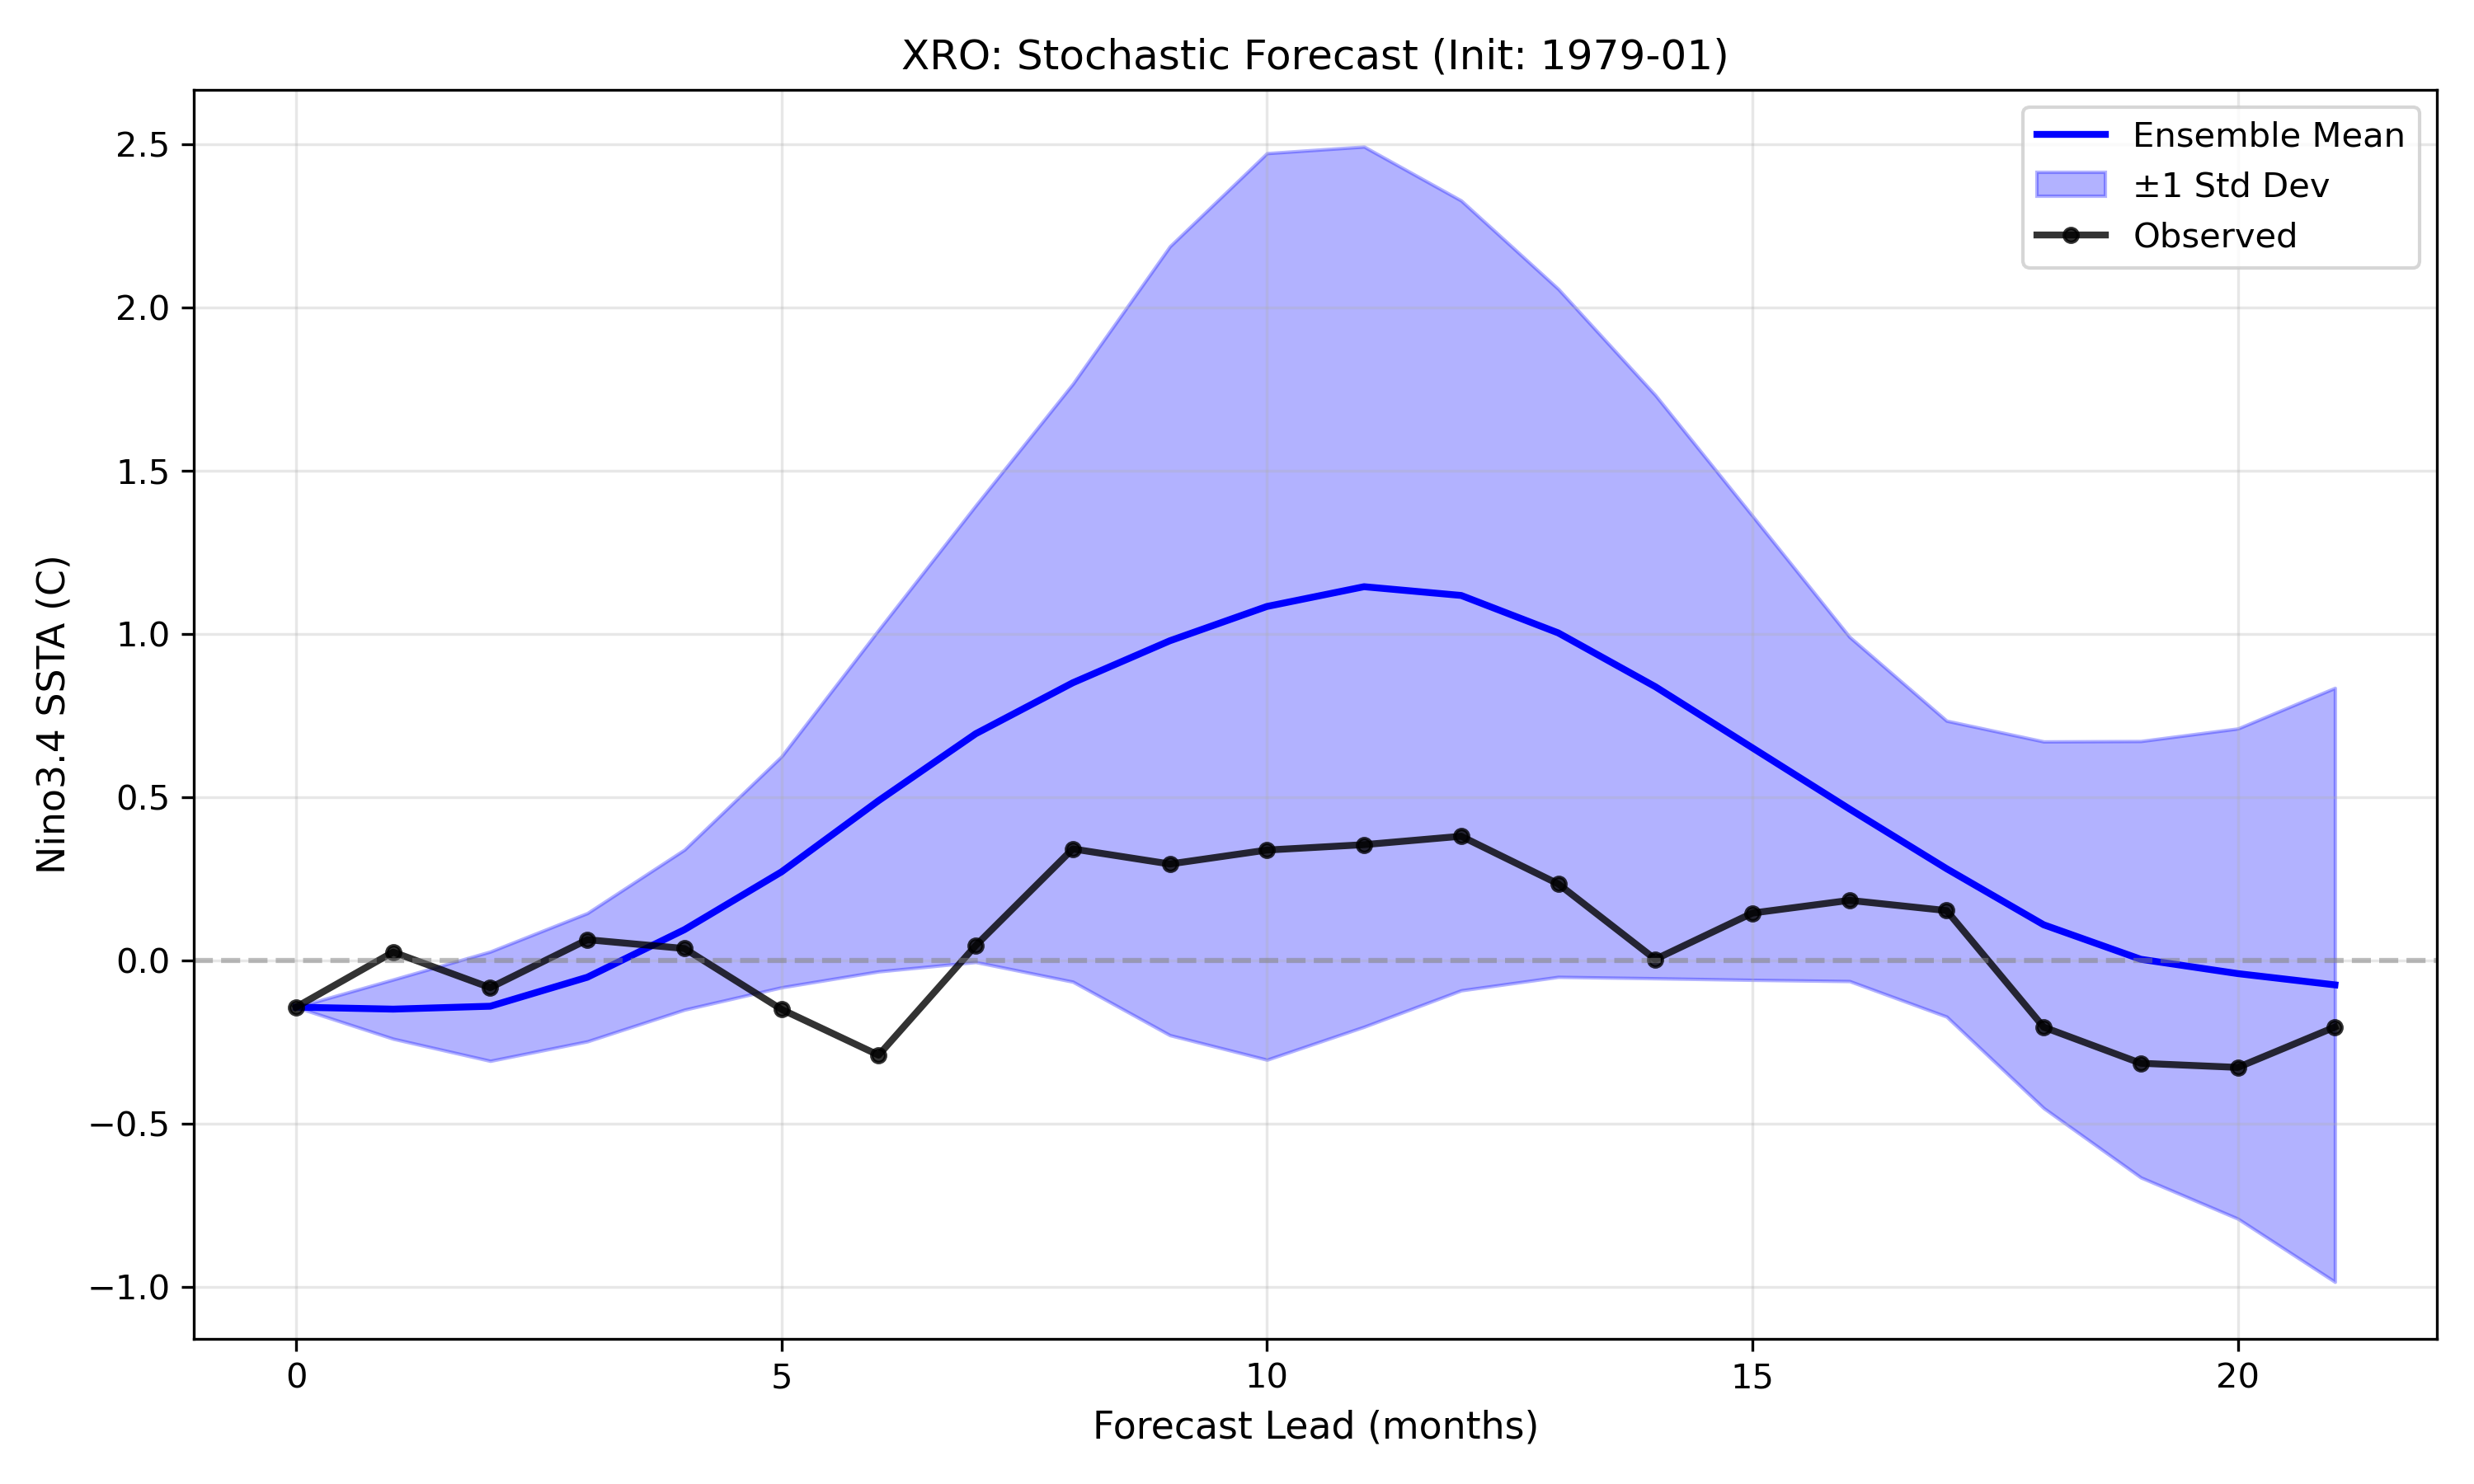
\includegraphics[width=0.48\textwidth]{forecast_XRO_outsample.png}
    \hfill
    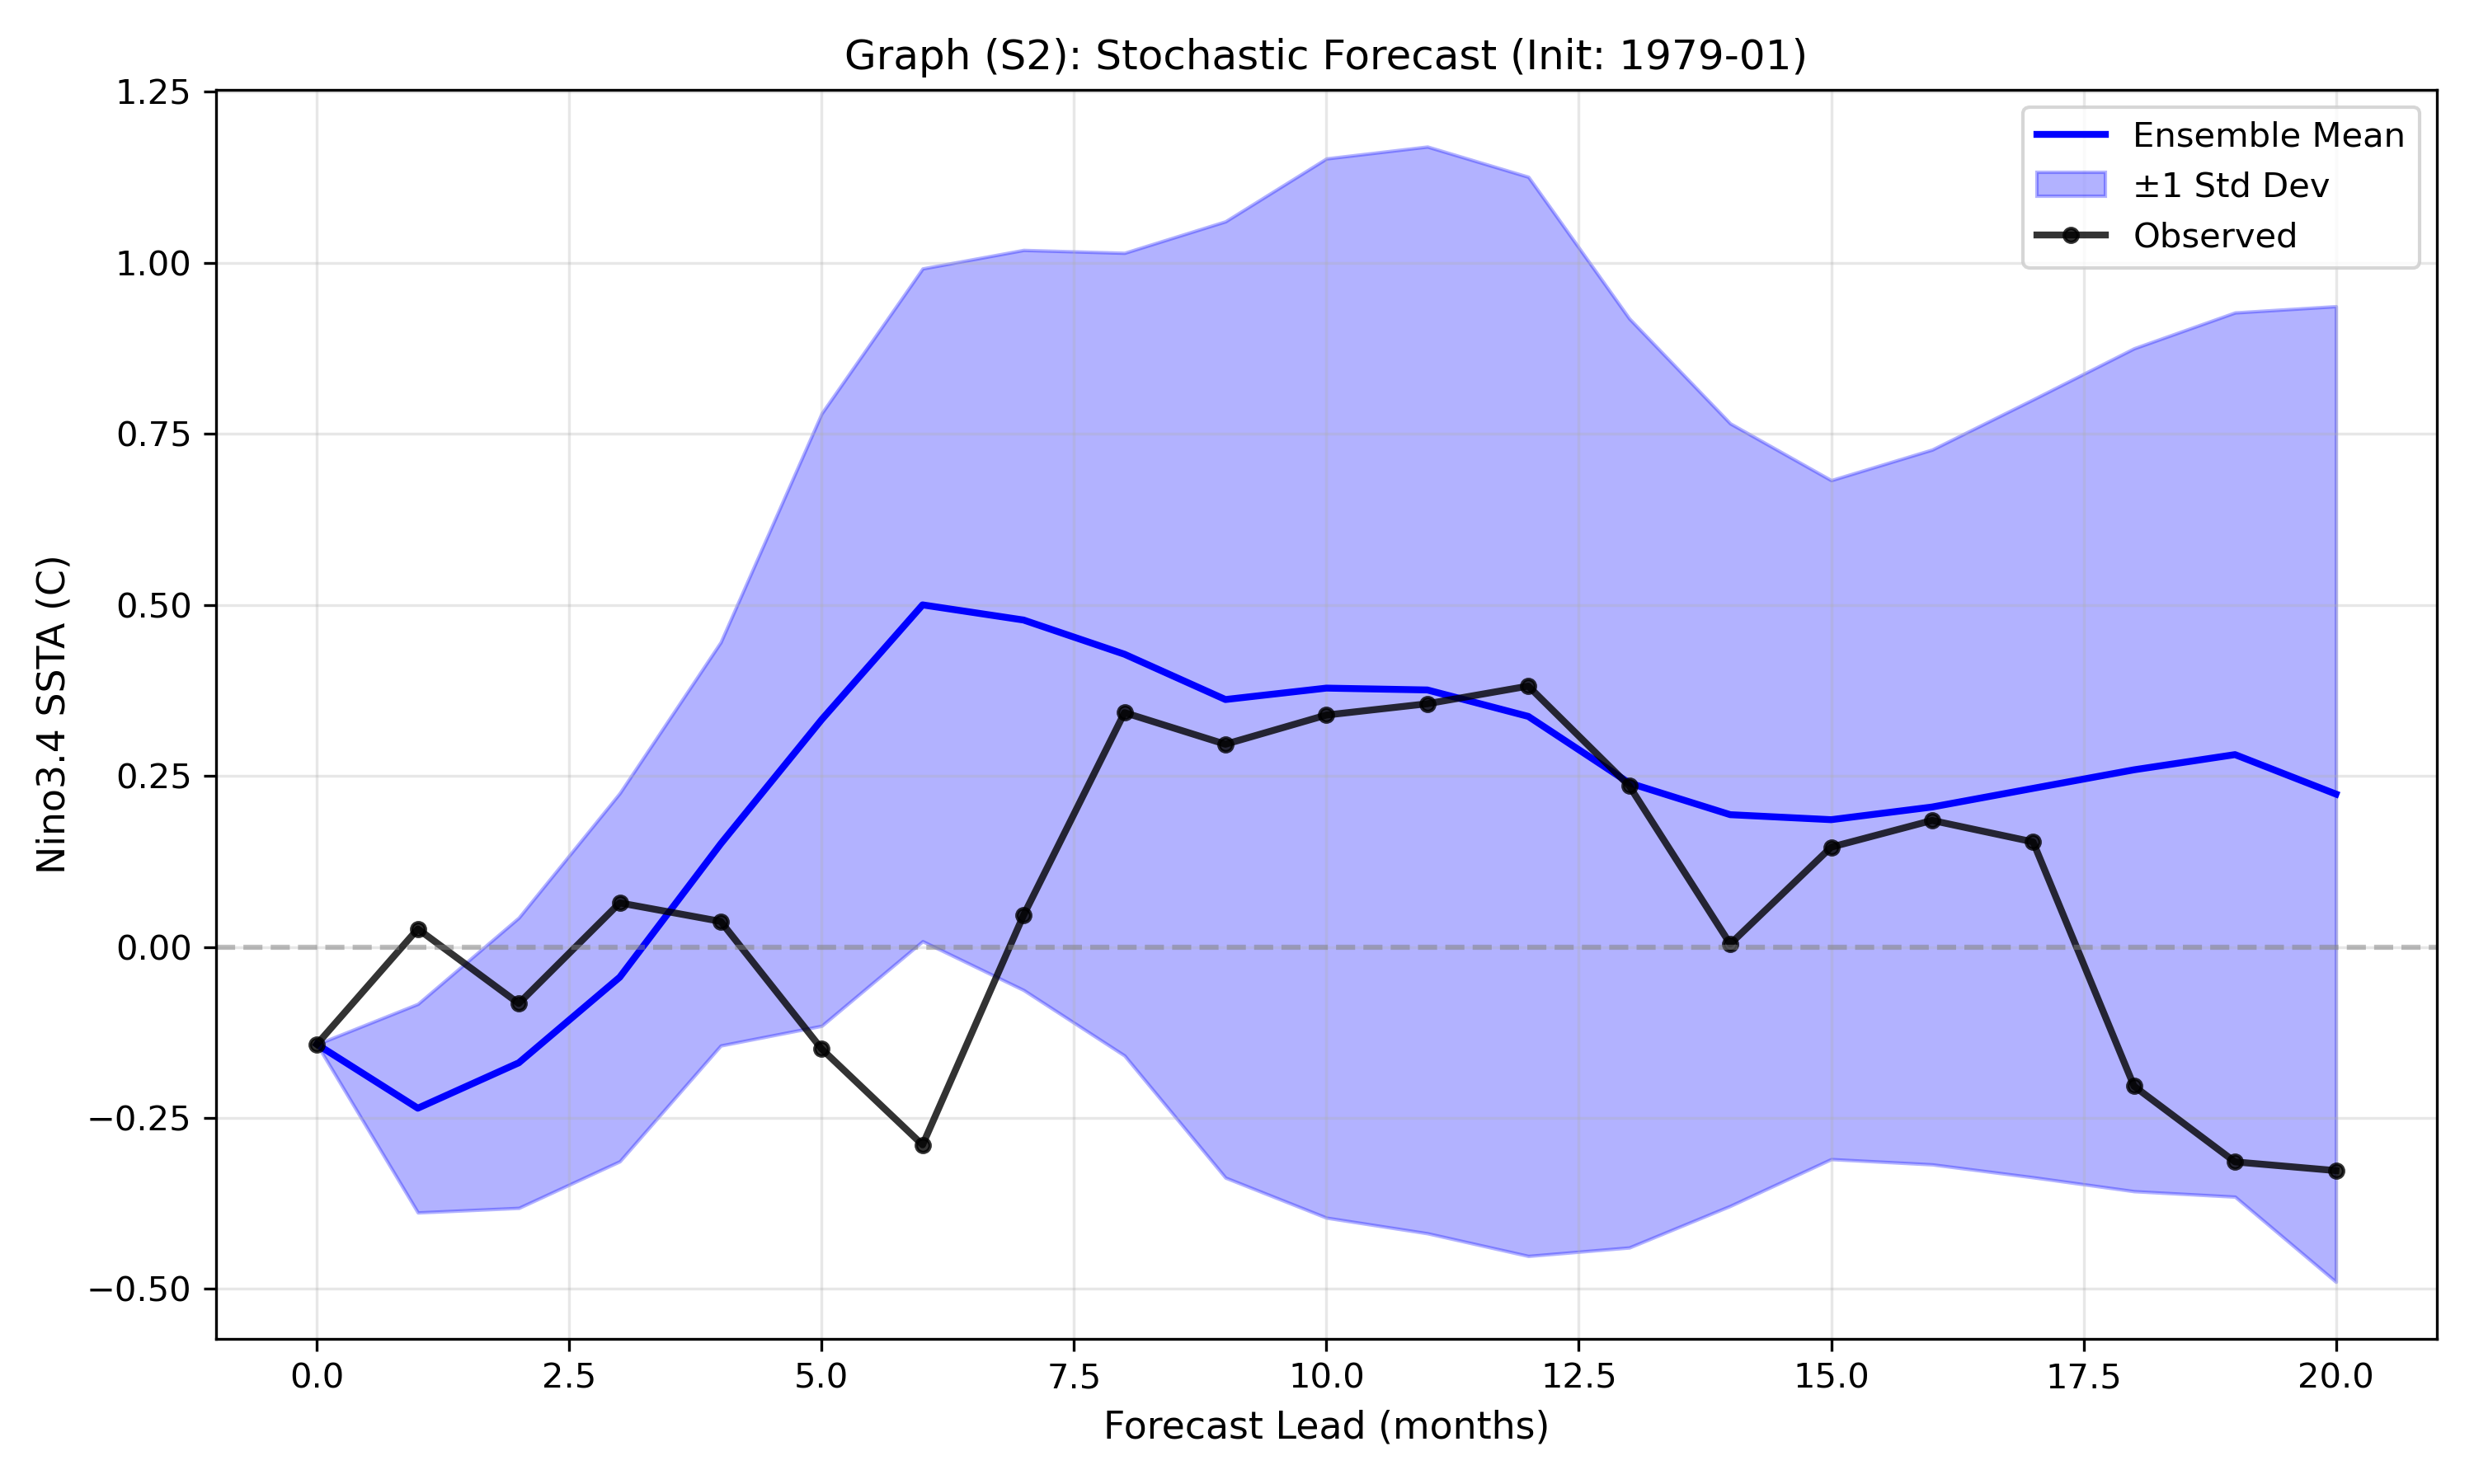
\includegraphics[width=0.48\textwidth]{forecast_Graph_S2_outsample.png}
    \caption{Ensemble forecast comparison. Left: XRO baseline with post-hoc noise. Right: NXRO-Graph with Stage 2 noise optimization. Shaded regions show 10--90\% quantile ranges; solid lines show ensemble median; dots show observations. The Stage 2 model exhibits wider, better-calibrated spread.}
    \label{fig:forecast_samples_outsample}
\end{figure}

Figure~\ref{fig:observed_nino34} displays the observed Ni\~no3.4 time series for context, highlighting major ENSO events during the study period. The 1997--98 El Ni\~no, the strongest on record~\cite{landsea2000springbarrier}, presents a particularly challenging forecast target due to its unprecedented amplitude.

\begin{figure}[htbp]
    \centering
    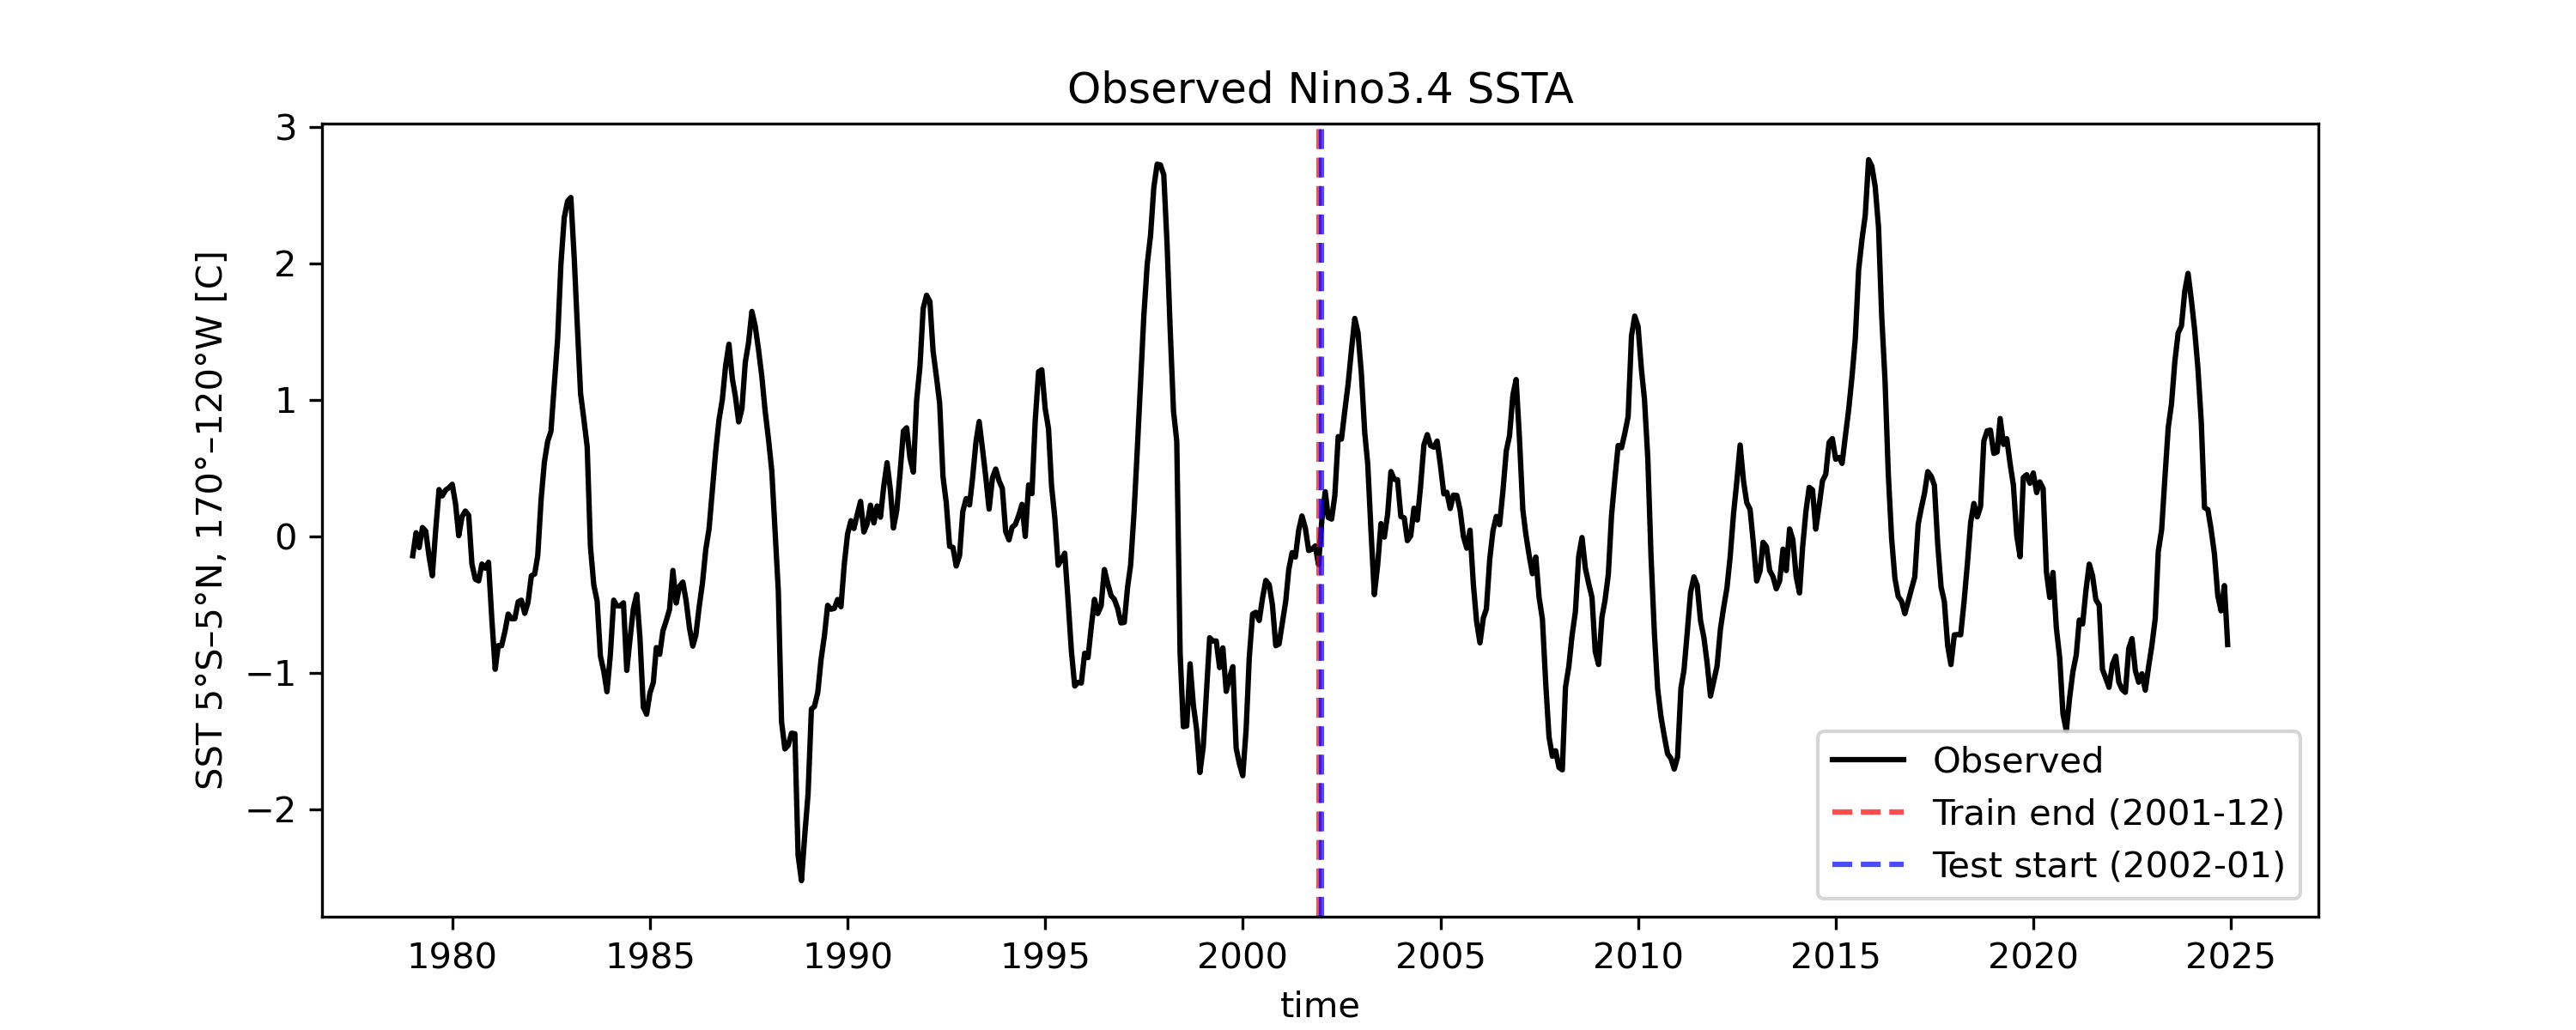
\includegraphics[width=0.9\textwidth]{NXRO_observed_Nino34_out_of_sample.png}
    \caption{Observed Ni\~no3.4 index from ORAS5 reanalysis~\cite{zuo2019oras5} (1979--2022). Major events include the 1982--83 and 1997--98 El Ni\~nos, the 2015--16 event, and extended La Ni\~na periods in 1998--2001 and 2020--2022.}
    \label{fig:observed_nino34}
\end{figure}

Figure~\ref{fig:plume_examples} presents forecast plumes for key ENSO events, comparing multiple NXRO variants against the XRO baseline. The forecasts initialized in April 1997 (before the major El Ni\~no) show all models predicting warming, though with varying amplitude and uncertainty. By December 1997 (peak of the event), the models show the transition toward La Ni\~na conditions that materialized in 1998.

\begin{figure}[htbp]
    \centering
    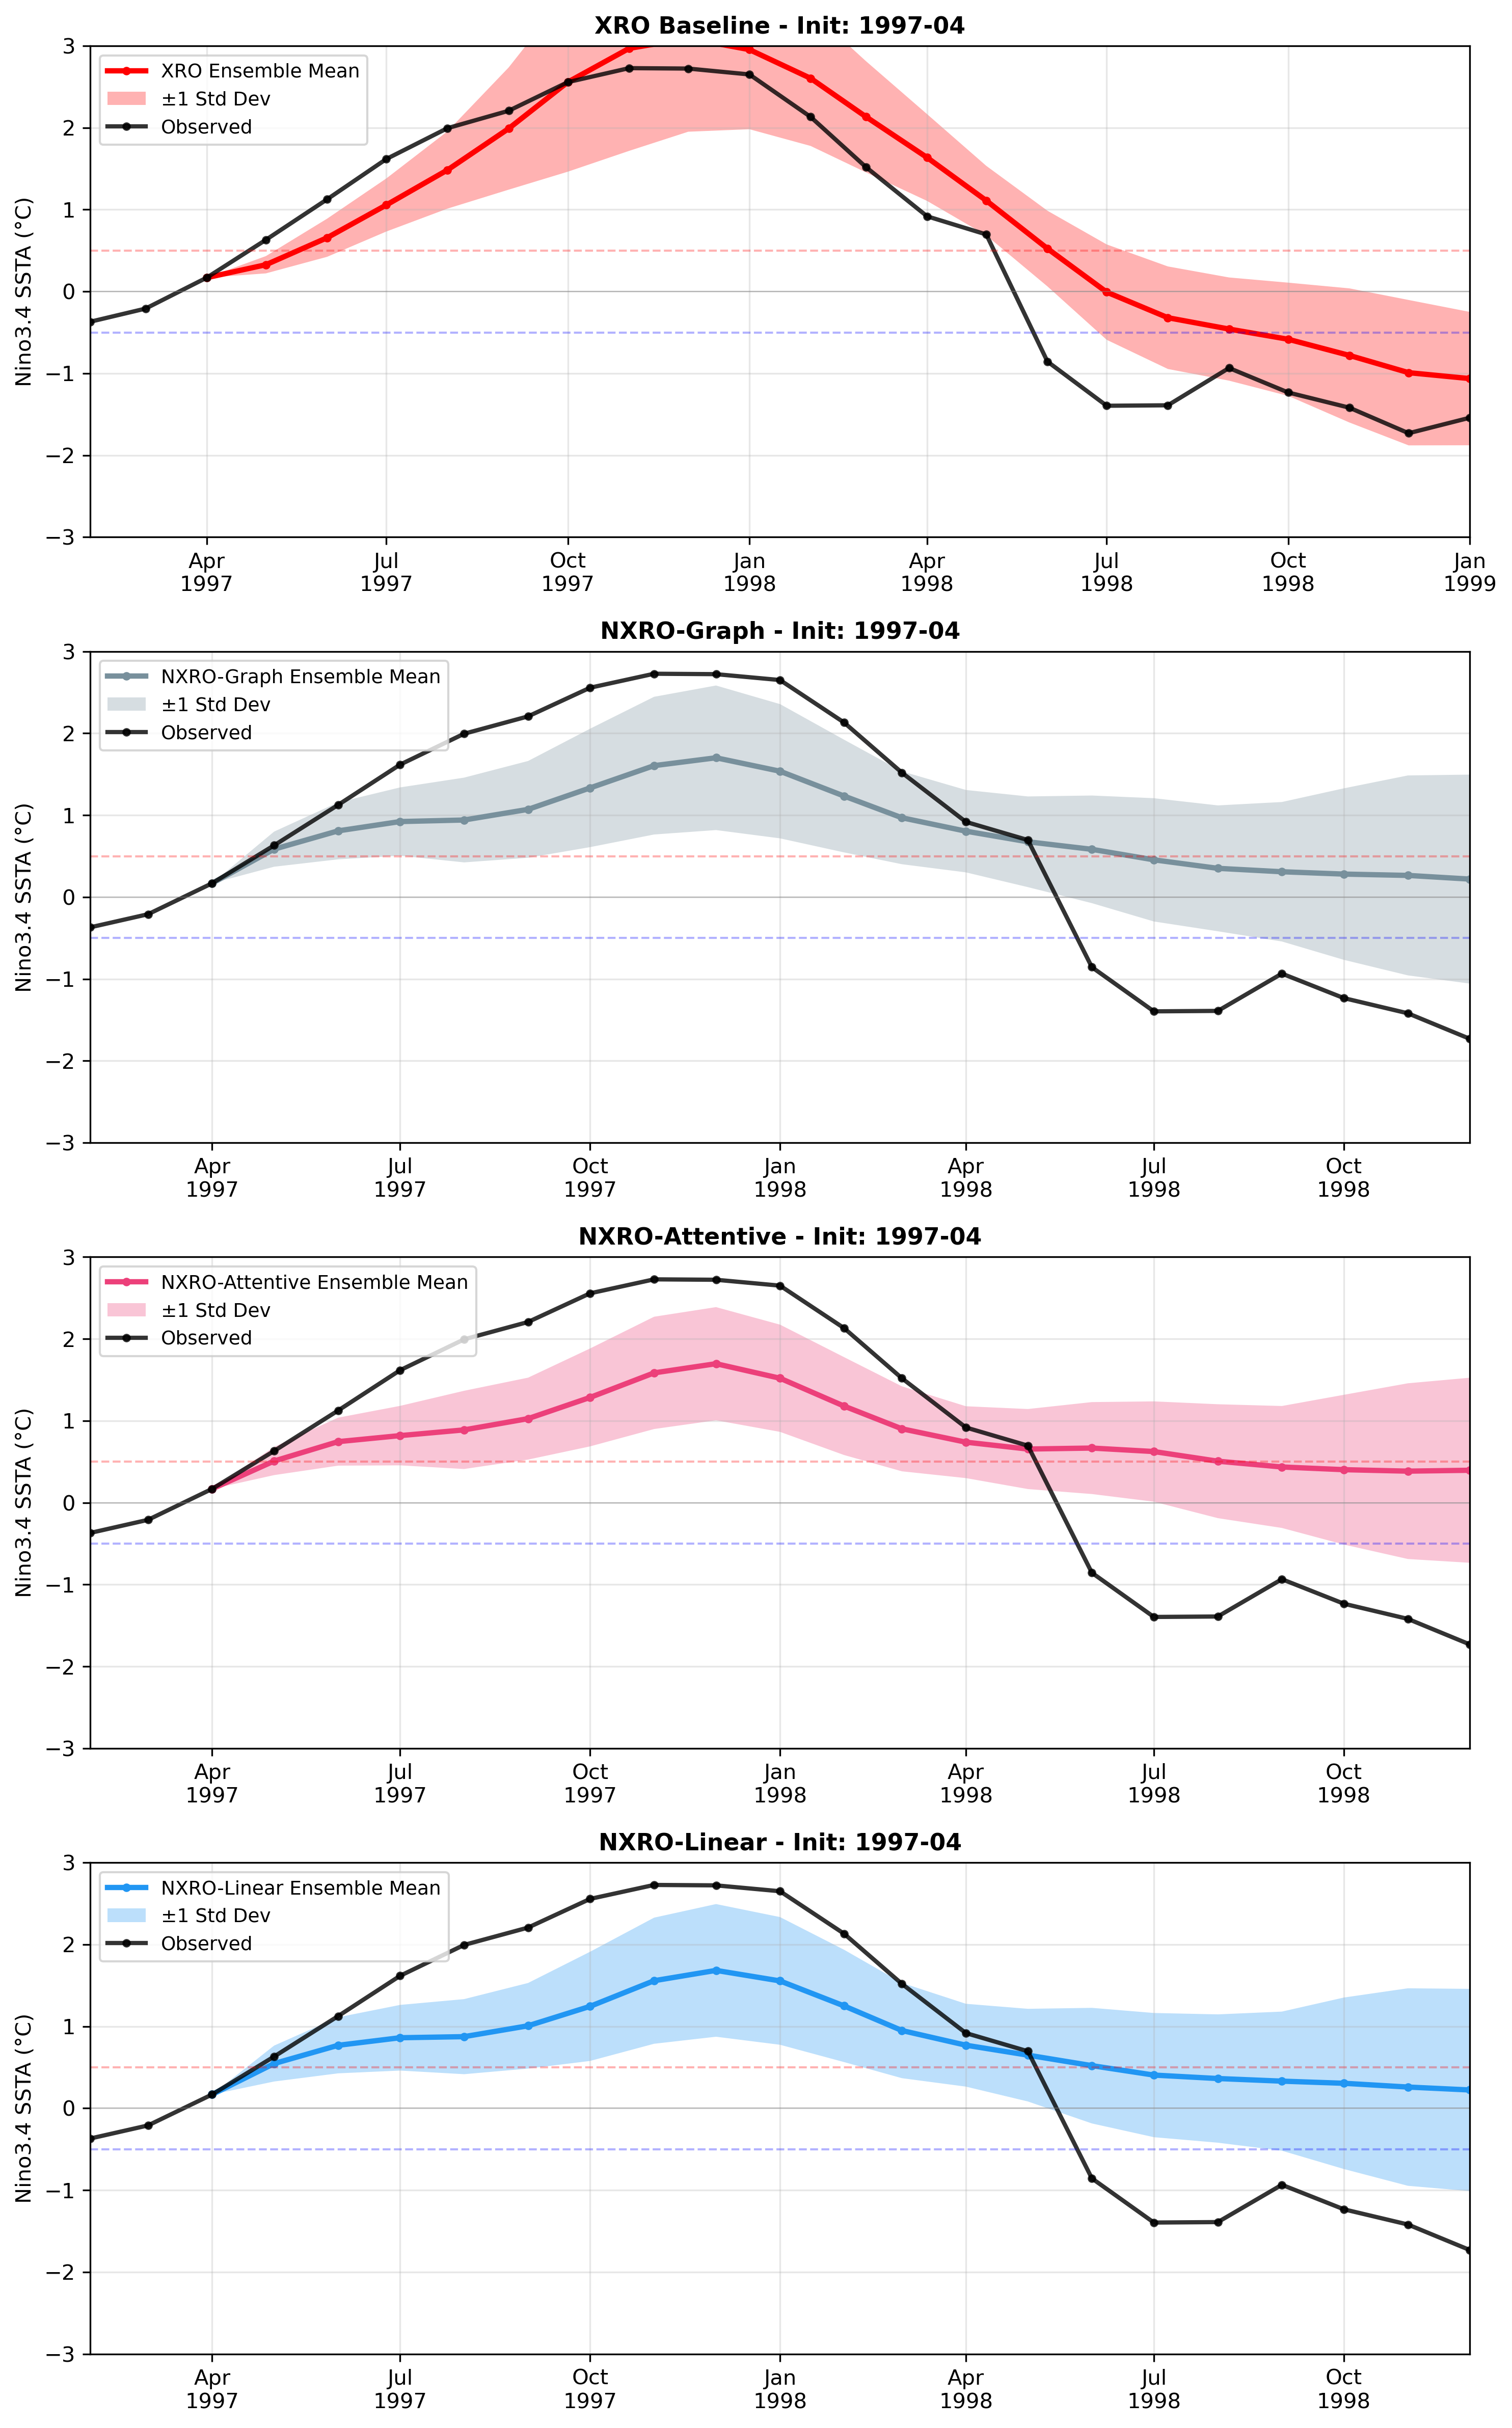
\includegraphics[width=0.48\textwidth]{plume_comparison_1997_04.png}
    \hfill
    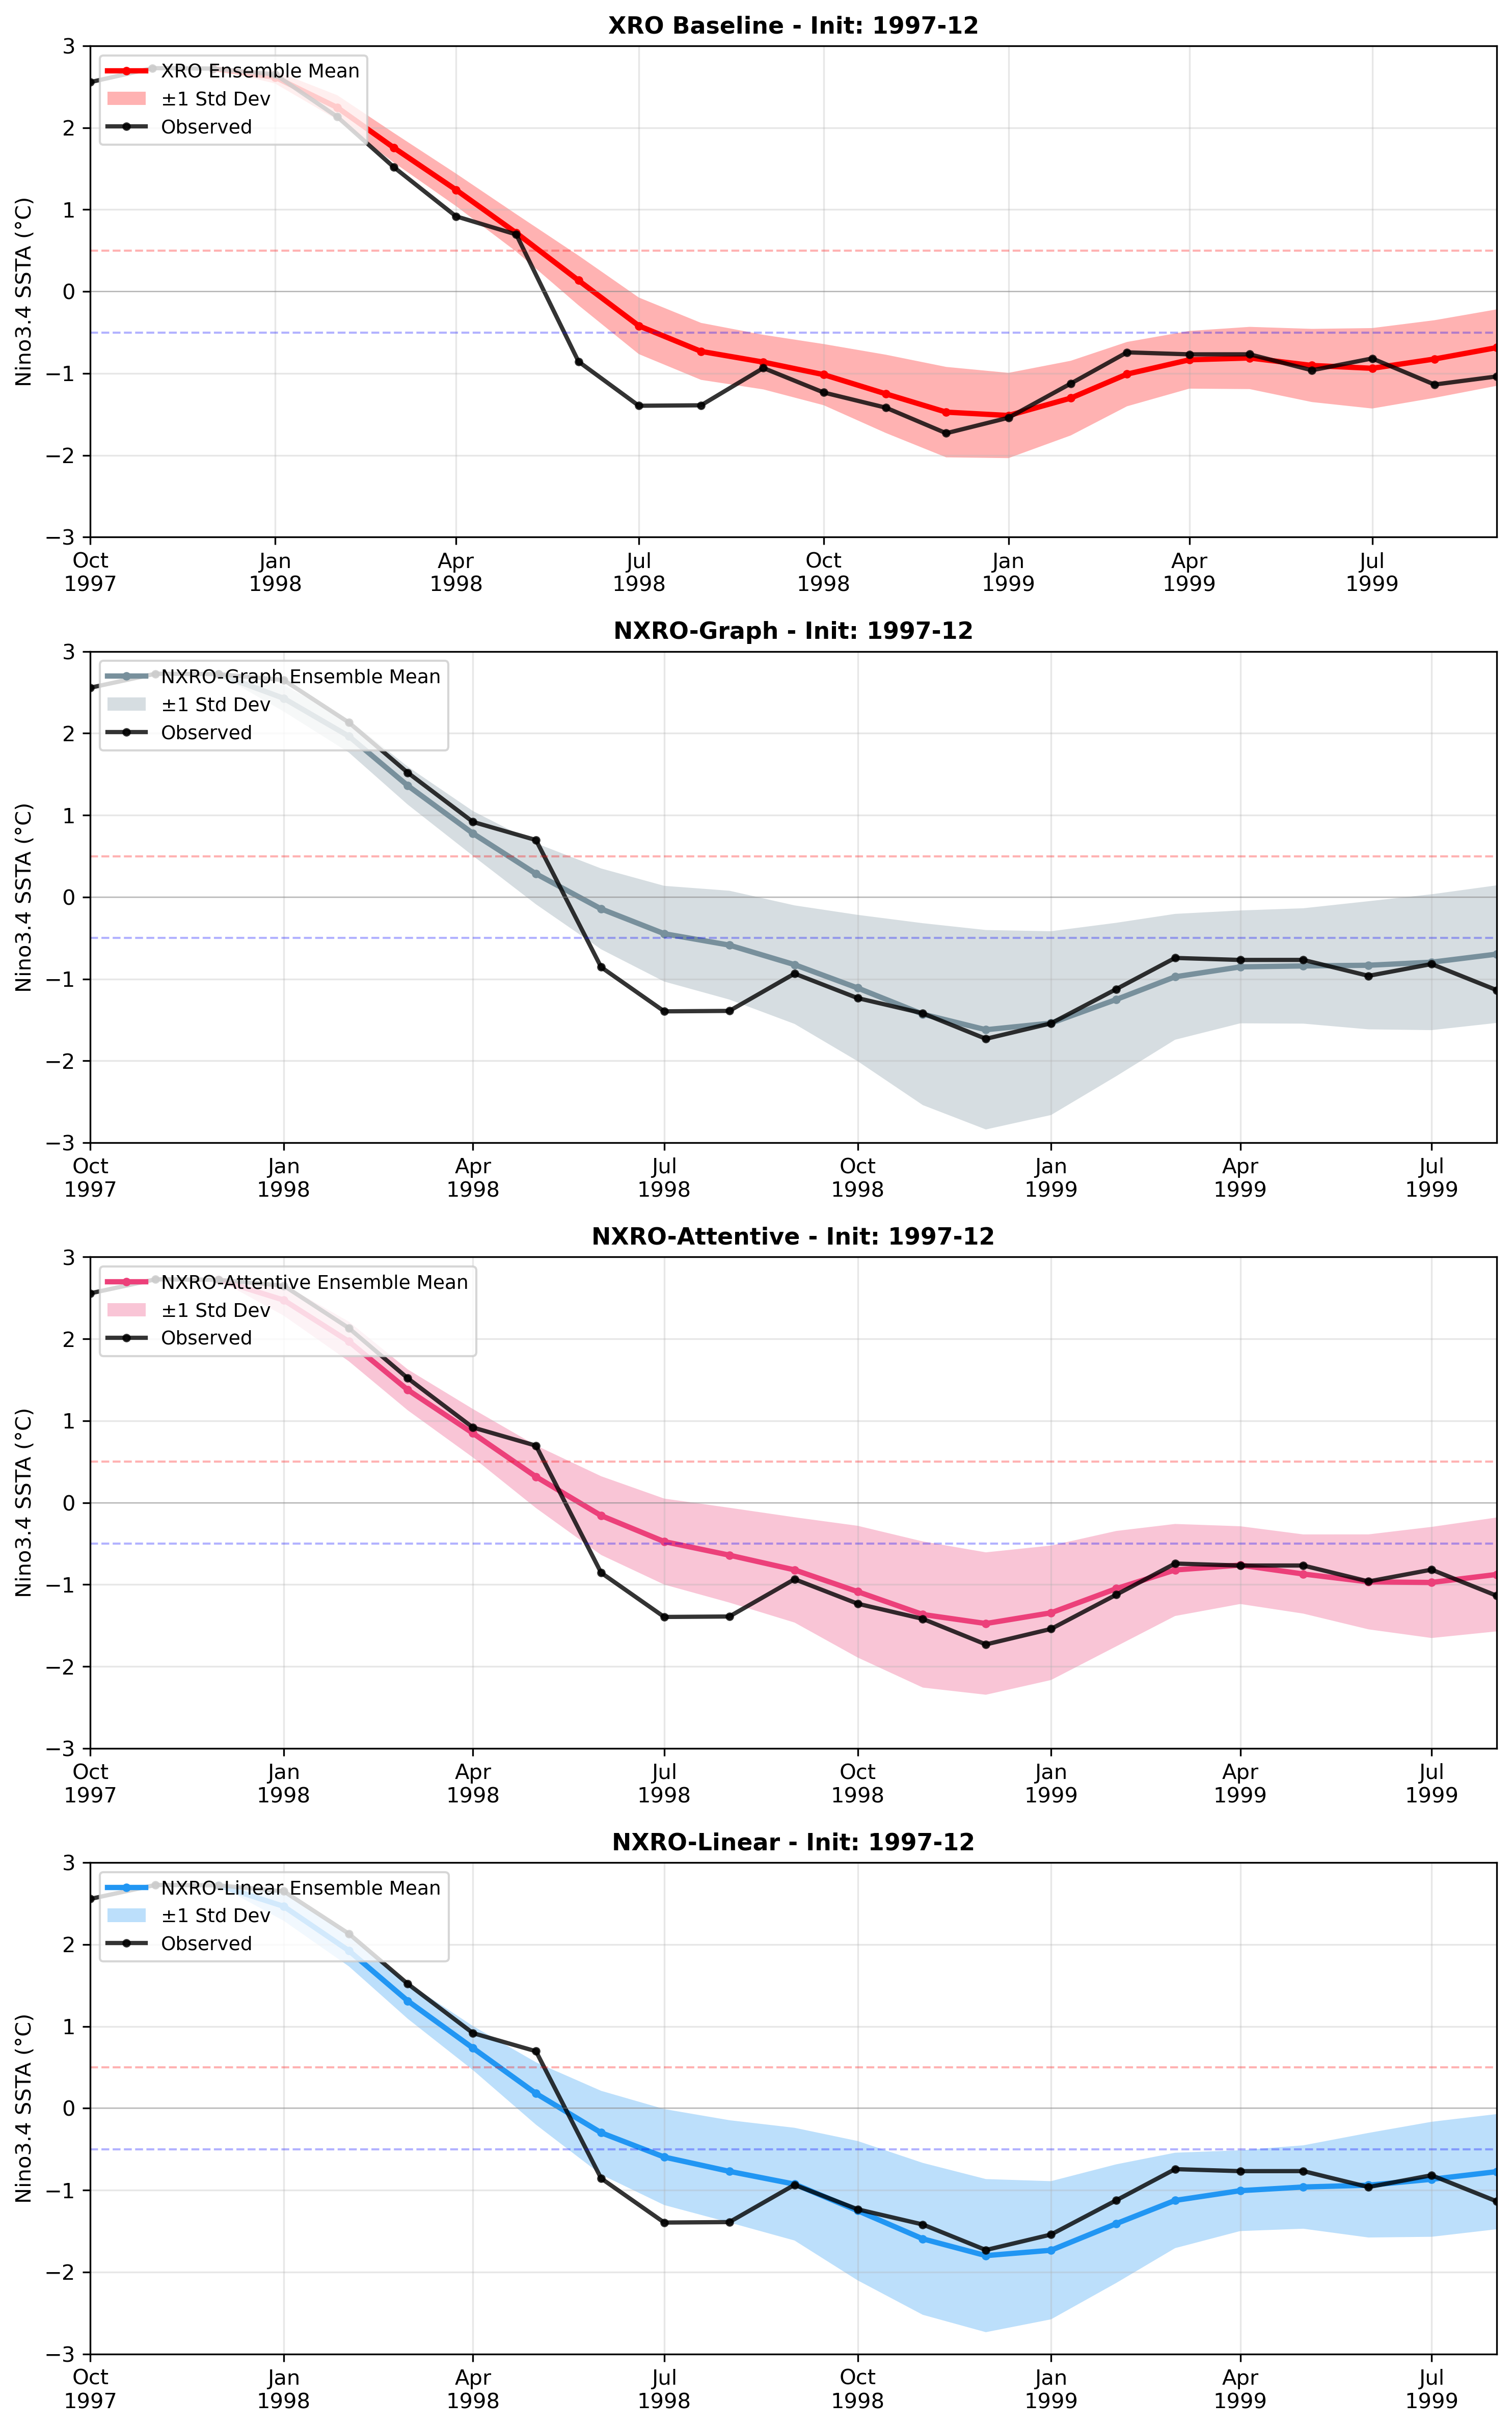
\includegraphics[width=0.48\textwidth]{plume_comparison_1997_12.png}
    \caption{Ensemble forecasts for the 1997--98 El Ni\~no. Left: Initialized April 1997, before the major warming. Right: Initialized December 1997, at peak El Ni\~no. Shaded regions show 10--90\% quantiles for each model.}
    \label{fig:plume_examples}
\end{figure}

\subsection{Summary}

Our stochastic forecasting experiments yield several conclusions relevant for probabilistic ENSO prediction, with implications for the broader challenge of uncertainty quantification in hybrid physics-ML models.

Likelihood-based noise optimization (Stage 2) consistently outperforms both the post-hoc fitting approach used by XRO~\cite{zhao2024xro} and climate model-derived noise. The key insight is that jointly optimizing AR(1) persistence and amplitude parameters via maximum likelihood produces better-calibrated ensembles than fitting each parameter independently. The 13\% CRPS improvement of the best model (NXRO-Graph) over XRO translates to meaningful gains for operational forecasting, and the improved calibration (spread-to-RMSE ratios of 0.63--0.68 versus 0.53 for XRO) provides more reliable uncertainty quantification.

The graph-based model achieves the best probabilistic forecast skill in the out-of-sample evaluation, with CRPS of 0.488 representing a 13\% improvement over XRO. This differs from the deterministic ranking where the residual model excelled, suggesting that the structured sparsity of the graph model provides particular benefits for uncertainty quantification.

Perhaps most importantly, our results demonstrate that climate model ensemble spread is not appropriate for calibrating neural forecast uncertainty---a cautionary finding for practitioners who might assume that established methods from numerical weather prediction~\cite{berner2017stochastic} transfer directly to machine learning settings. The structural biases captured by observation-simulation differences are irrelevant for well-optimized neural models, leading to severely over-dispersed ensembles. When a forecast model has been optimized to match observations, practitioners should calibrate uncertainty from model residuals rather than external sources.

These findings suggest a general principle: uncertainty quantification methods must be matched to the properties of the prediction model. Approaches designed for physics-based models with known structural limitations require adaptation when applied to flexible machine learning models that minimize prediction error through optimization. This insight aligns with recent work on time-aware neural ODEs~\cite{zhang2023timeaware} and hybrid dynamical systems~\cite{oh2024dualdynamics}, which demonstrate that effective uncertainty quantification requires careful consideration of the model's data-fitting capacity.


\section{Conclusion}
\label{sec:conclusion}

We have presented the Neural Residual ODE (NXRO) framework for ENSO forecasting, systematically investigating how to combine physics-based structure with machine learning flexibility for climate prediction under severe data limitations. Our experiments, spanning 43 model variants evaluated on rigorous out-of-sample forecasting, yield insights relevant to both the climate science and machine learning communities.

\subsection{Principal Findings}

The central result of this work is that simpler hybrid architectures outperform both the full physics-based XRO model and pure deep learning approaches. The residual neural model, which combines a seasonal linear operator with a three-layer MLP, achieves the best deterministic forecast skill with test RMSE of 0.567°C---a 6.3\% improvement over the XRO baseline. This model omits the polynomial nonlinearities that are central to XRO's physics-based formulation, suggesting that the rigid polynomial basis may capture training-period patterns that do not generalize to future data.

The success of the linear-only variant, which outranks XRO despite having no nonlinear terms, reinforces this conclusion. With only 23 years of training data, the regularization provided by architectural simplicity outweighs the representational benefits of polynomial nonlinearities. The XRO model's variable-by-variable closed-form fitting, while computationally convenient, does not find globally optimal coefficients for multi-step forecasting. Joint gradient-based optimization, even with identical model structure, yields better generalization.

The graph-based and attention-based models demonstrate that structured sparsity provides effective regularization without sacrificing expressiveness. By restricting interactions to follow physics-informed patterns---either through fixed graph connectivity derived from XRO or through learned attention with masking---these models achieve competitive deterministic performance and excel at probabilistic forecasting.

The transformer-based model's failure ranks among our most important findings. Despite transformers' remarkable success in natural language processing~\cite{vaswani2017attention} and computer vision~\cite{dosovitskiy2020image}, the architecture performs worse than the physics-based XRO baseline on our climate forecasting task. This result carries implications for practitioners: modern deep learning architectures do not automatically transfer to small-data scientific domains. The approximately 300 monthly observations in our training set are insufficient for transformers to learn the seasonal structure, teleconnection patterns, and amplitude-dependent dynamics that the physics-informed linear operator encodes architecturally.

For probabilistic forecasting, likelihood-based noise optimization (Stage 2) consistently outperforms both post-hoc fitting and climate model-derived noise. The graph-based model with Stage 2 noise achieves CRPS of 0.488, representing a 13\% improvement over XRO. Equally important, the calibration improves substantially: spread-to-RMSE ratios increase from 0.53 (XRO) to 0.65 (NXRO-Graph), providing more reliable uncertainty quantification for decision-making applications.

The failure of climate model ensemble spread (Stage 3) to calibrate neural forecast uncertainty reveals a fundamental mismatch. The structural biases and parameterization differences captured by observation-simulation differences are irrelevant for well-optimized neural models that have already minimized prediction error. Uncertainty quantification methods must be matched to the properties of the prediction model.

\subsection{Broader Implications}

Our results speak to ongoing debates about the role of physics in machine learning for science~\cite{karniadakis2021physics,willard2022integrating}. The hybrid approach---encoding well-understood physics as architectural structure while learning corrections from data~\cite{rackauckas2020universal,yin2021augmenting}---emerges as the optimal strategy for the small-data regime characteristic of climate science and many other scientific domains.

Physics provides sample-efficient inductive bias~\cite{bronstein2021geometric}. The seasonal linear operator captures the dominant ENSO dynamics with far fewer parameters than a neural network would require to learn equivalent structure from data. This efficiency is critical when training samples number in the hundreds rather than millions, a regime where geometric and physical priors become essential for generalization.

Machine learning provides flexibility where physics is uncertain. The MLP residual, graph convolution, or attention mechanism can capture dynamics that the polynomial basis misses without requiring the modeler to specify functional forms a priori. The learned components adapt to the specific dataset rather than imposing assumptions that may not hold.

End-to-end optimization aligns training with the ultimate objective. By optimizing for multi-step forecast skill rather than one-step prediction error, the gradient-based approach finds coefficient configurations that minimize error accumulation over extended integration periods. This differs fundamentally from traditional fitting approaches that optimize each component independently.

The tension between model capacity and generalization requires careful navigation. Our experiments reveal that models achieving the best training performance often exhibit the largest generalization gaps. The art of hybrid modeling lies in providing sufficient flexibility to capture real dynamics while constraining the hypothesis space enough to prevent overfitting.

\subsection{Recommendations}

Based on our comprehensive evaluation, we offer guidance for practitioners developing ENSO forecast systems.

For operational deterministic forecasting, the residual neural model (NXRO-Res) trained directly on observations represents the recommended default. Its combination of physics-informed linear structure and flexible neural residual achieves the best out-of-sample skill while remaining computationally efficient and straightforward to train. Pre-training on climate model simulations does not improve and may degrade performance for this architecture.

For probabilistic forecasting, the graph-based model (NXRO-Graph) with Stage 2 noise optimization provides the best ensemble forecasts. The structured sparsity of the graph convolution appears particularly beneficial for uncertainty quantification, yielding both lower CRPS and better calibration than the residual model.

For applications requiring interpretable coupling patterns, the linear-only model (NXRO-Linear) or physics-structured model with frozen RO terms (NXRO-FixRO) preserve the interpretability of traditional approaches while benefiting from gradient-based optimization of the linear operator.

For two-stage transfer learning from climate model simulations, the pure neural ODE or physics-structured models benefit most from pre-training. The residual model's flexible MLP component may learn simulation-specific biases that are difficult to unlearn during fine-tuning on observations.

Regardless of architecture choice, rigorous out-of-sample evaluation is essential for model selection. In-sample metrics systematically favor complex models that overfit, providing misleading guidance about operational performance. Any evaluation of forecast systems should employ temporal holdout spanning multiple ENSO cycles.


\section{Limitations and Future Directions}
\label{sec:future}

While our results demonstrate the promise of hybrid physics-ML approaches for ENSO forecasting, several limitations of the current work suggest directions for future research.

\subsection{Data and Evaluation Limitations}

Our evaluation relies on a single train-test split (1979--2001 for training, 2002--2022 for testing), which provides a rigorous out-of-sample assessment but does not characterize variability across different climate regimes. The training period includes the major 1982--83 and 1997--98 El Ni\~no events, while the test period includes the 2015--16 event and extended La Ni\~na conditions of 2020--2022. Model rankings might differ with alternative splits that allocate these events differently.

Rolling-window cross-validation would provide more robust model selection by averaging performance across multiple train-test splits. However, the relatively short observational record (44 years) limits the number of independent folds possible while maintaining sufficient training data. Extending the analysis to earlier periods using reconstructed indices would expand the available data but introduce additional uncertainty from the reconstruction methodology.

The current framework uses only ORAS5~\cite{zuo2019oras5} reanalysis for training and evaluation. Multiple reanalysis products (ERA5~\cite{hersbach2020era5}, GODAS, SODA) provide alternative representations of the historical climate state, each with distinct biases and uncertainty characteristics. Training on multiple products or evaluating across products would assess robustness to observational uncertainty. Our codebase supports multi-dataset evaluation, but systematic comparison remains for future work.

\subsection{Architectural Extensions}

The transformer failure in our experiments does not preclude success with modified architectures or training procedures. Recent work on reservoir computing for El Ni\~no prediction~\cite{guardamagna2025reservoir} demonstrates that alternative recurrent architectures can achieve high skill, suggesting that the key limitation is not recurrence per se but the combination of architecture, data volume, and inductive biases. Several remediation strategies merit investigation.

Pre-training on large climate model ensembles before fine-tuning on observations could provide transformers with the data volume they require. CMIP6~\cite{eyring2016cmip6} simulations span thousands of model-years across 100+ models, offering abundant data with realistic (though not identical) ENSO dynamics. The challenge lies in the domain shift between simulated and observed climate, which our residual model experiments suggest can be detrimental for flexible architectures.

Physics-informed attention mechanisms could encode domain knowledge as architectural constraints. Rather than allowing unrestricted self-attention, the attention weights could be masked or regularized to follow known teleconnection patterns, similar to our NXRO-Attentive model but applied within a full transformer architecture.

Hybrid transformer architectures that retain the physics-informed linear operator while using transformer layers only for the residual might combine the benefits of both approaches. The linear operator would provide the inductive bias needed for small-data learning, while the transformer would offer flexible capacity for capturing complex residual dynamics.

For graph-based models, allowing the adjacency matrix to be learned during training rather than fixed from XRO could discover novel teleconnection patterns, similar to data-driven discovery of coordinates and governing equations~\cite{champion2019data}. Sparsity-inducing regularization would be necessary to prevent the learned graph from becoming fully connected. Multi-scale graph architectures with hierarchical structure could capture both local interactions and long-range teleconnections. Additionally, Neural Flows~\cite{bilos2021neural} offer a computationally efficient alternative to Neural ODEs that could enable scaling to higher-dimensional state spaces.

\subsection{Stochastic Modeling Extensions}

The Stage 3 failure reveals that climate model ensemble spread does not directly transfer to neural forecast uncertainty, but modifications might recover its value. Scaling the simulation-derived noise by a learned factor ($\sigma_{\text{scaled}} = \alpha \cdot \sigma_{\text{simulations}}$ with $\alpha \ll 1$) could reduce the over-dispersion while retaining information about structural uncertainty. The scaling factor could be optimized via the same likelihood objective used in Stage 2.

Selecting a subset of high-quality simulations rather than using all 100 CMIP6 members might improve Stage 3 performance. Ensemble members with smaller biases relative to observations would contribute noise estimates more relevant for well-tuned neural models. Alternatively, using only ensemble reanalyses (such as ERA5-ens or ORAS5-ens) that share the observational constraints of the training data could reduce the distribution mismatch.

Hybrid noise models that combine residual-based and simulation-based uncertainty could capture both aleatoric uncertainty (from atmospheric noise, represented by model residuals) and epistemic uncertainty (from structural model limitations, represented by simulation spread). The relative weighting could vary with lead time, with residual-based uncertainty dominating at short leads and simulation-based uncertainty becoming more relevant at long leads where model structural errors accumulate.

Deep ensembles~\cite{lakshminarayanan2017simple}---training multiple NXRO models with different random initializations---provide an alternative approach to epistemic uncertainty quantification that does not rely on external simulations. The spread across ensemble members captures uncertainty arising from the non-convex optimization landscape and finite training data.

\subsection{Interpretability and Scientific Discovery}

The learned components of NXRO models encode information about climate dynamics that could yield scientific insights beyond forecast improvement.

The attention weights in NXRO-Attentive reveal which climate modes the model considers relevant for predicting each variable at each time step. Visualizing these attention patterns across different ENSO phases could discover state-dependent teleconnection relationships not captured by the static linear operator. Comparisons with physical understanding of ENSO dynamics would validate whether the learned patterns correspond to known mechanisms or suggest novel hypotheses.

The graph convolution weights in NXRO-Graph provide interpretable coupling strengths between climate indices. Comparing these learned weights to the XRO-derived adjacency and to physical coupling estimates from recharge oscillator theory could identify discrepancies that reveal limitations of current physical understanding.

The MLP residual in NXRO-Res captures dynamics that the linear operator misses. Analyzing the residual's dependence on state amplitude, season, and climate mode configuration could identify the functional forms of missing nonlinearities. If the residual approximates specific polynomial or other structured functions, this would suggest extensions to the XRO basis.

\subsection{Operational Considerations}

Deploying NXRO models for operational ENSO forecasting requires addressing practical considerations beyond forecast skill.

Real-time forecasting pipelines must handle data latency, quality control, and automated retraining as new observations become available. The computational efficiency of NXRO models (training in minutes on standard hardware, inference in milliseconds) makes operational deployment feasible, but robust software infrastructure is necessary.

Communicating probabilistic forecasts to decision-makers requires careful attention to visualization and uncertainty representation. The ensemble plumes shown in our results provide one approach, but alternative representations (probability of exceedance curves, categorical probability forecasts) may better serve specific applications in agriculture, water management, or disaster preparedness.

Comparison with operational forecast centers (IRI, CPC, ECMWF, JMA) would contextualize NXRO performance relative to state-of-the-art dynamical and statistical systems. Such comparisons require real-time forecast submission and evaluation over multiple years to assess skill in operational conditions rather than retrospective analysis.

\subsection{Broader Applications}

The NXRO framework extends naturally to other climate forecasting problems where physics-based models exist but have known limitations.

The Indian Ocean Dipole~\cite{saji1999dipole} exhibits recharge-oscillator dynamics similar to ENSO, with thermocline depth anomalies in the eastern Indian Ocean driving SST variability. Adapting NXRO to IOD prediction would require redefining the state variables and potentially the RO nonlinear basis, but the core framework of physics-informed linear dynamics plus neural residual would apply directly.

The Atlantic Multi-decadal Oscillation operates on longer timescales (60--80 years), presenting challenges for training and evaluation given the limited observational record. Transfer learning from climate model simulations might be more valuable for AMO than for ENSO, as the models provide the only source of multiple complete cycles.

Sub-seasonal to seasonal (S2S) prediction~\cite{vitart2017subseasonal} of temperature and precipitation anomalies represents a broader application domain where ENSO serves as a source of predictability. Extending NXRO to predict regional climate impacts conditioned on ENSO state would connect the framework to applications with direct societal relevance.

Finally, the hybrid physics-ML approach embodied by NXRO has potential beyond climate science. Any domain with well-understood but imperfect physics---fluid dynamics, molecular simulation, epidemiology---could benefit from architectures that encode physical structure while learning corrections from data~\cite{daw2022physics,beucler2021enforcing}. The principles we have identified---physics provides sample-efficient inductive bias, ML provides flexibility, end-to-end optimization aligns training with objectives---appear general rather than domain-specific, as evidenced by the success of similar hybrid approaches across scientific domains~\cite{willard2022integrating,yin2021augmenting}.


\bibliographystyle{plain}
\bibliography{references}

\end{document}
